\PassOptionsToPackage{unicode=true}{hyperref} % options for packages loaded elsewhere
\PassOptionsToPackage{hyphens}{url}
%
\documentclass[]{book}
\usepackage{lmodern}
\usepackage{amssymb,amsmath}
\usepackage{ifxetex,ifluatex}
\usepackage{fixltx2e} % provides \textsubscript
\ifnum 0\ifxetex 1\fi\ifluatex 1\fi=0 % if pdftex
  \usepackage[T1]{fontenc}
  \usepackage[utf8]{inputenc}
  \usepackage{textcomp} % provides euro and other symbols
\else % if luatex or xelatex
  \usepackage{unicode-math}
  \defaultfontfeatures{Ligatures=TeX,Scale=MatchLowercase}
\fi
% use upquote if available, for straight quotes in verbatim environments
\IfFileExists{upquote.sty}{\usepackage{upquote}}{}
% use microtype if available
\IfFileExists{microtype.sty}{%
\usepackage[]{microtype}
\UseMicrotypeSet[protrusion]{basicmath} % disable protrusion for tt fonts
}{}
\IfFileExists{parskip.sty}{%
\usepackage{parskip}
}{% else
\setlength{\parindent}{0pt}
\setlength{\parskip}{6pt plus 2pt minus 1pt}
}
\usepackage{hyperref}
\hypersetup{
            pdftitle={DAEs},
            pdfauthor={Jan Heiland},
            pdfborder={0 0 0},
            breaklinks=true}
\urlstyle{same}  % don't use monospace font for urls
\usepackage{longtable,booktabs}
% Fix footnotes in tables (requires footnote package)
\IfFileExists{footnote.sty}{\usepackage{footnote}\makesavenoteenv{longtable}}{}
\usepackage{graphicx,grffile}
\makeatletter
\def\maxwidth{\ifdim\Gin@nat@width>\linewidth\linewidth\else\Gin@nat@width\fi}
\def\maxheight{\ifdim\Gin@nat@height>\textheight\textheight\else\Gin@nat@height\fi}
\makeatother
% Scale images if necessary, so that they will not overflow the page
% margins by default, and it is still possible to overwrite the defaults
% using explicit options in \includegraphics[width, height, ...]{}
\setkeys{Gin}{width=\maxwidth,height=\maxheight,keepaspectratio}
\setlength{\emergencystretch}{3em}  % prevent overfull lines
\providecommand{\tightlist}{%
  \setlength{\itemsep}{0pt}\setlength{\parskip}{0pt}}
\setcounter{secnumdepth}{5}
% Redefines (sub)paragraphs to behave more like sections
\ifx\paragraph\undefined\else
\let\oldparagraph\paragraph
\renewcommand{\paragraph}[1]{\oldparagraph{#1}\mbox{}}
\fi
\ifx\subparagraph\undefined\else
\let\oldsubparagraph\subparagraph
\renewcommand{\subparagraph}[1]{\oldsubparagraph{#1}\mbox{}}
\fi

% set default figure placement to htbp
\makeatletter
\def\fps@figure{htbp}
\makeatother

\usepackage{booktabs}
\usepackage{xcolor}
\definecolor{jhsc}{HTML}{1f57c7}
\newenvironment {JHSAYS} [0] {\begin{quote}\color{jhsc}} {\end{quote}}
\setcounter{MaxMatrixCols}{20}
\usepackage{booktabs}
\usepackage{longtable}
\usepackage{array}
\usepackage{multirow}
\usepackage{wrapfig}
\usepackage{float}
\usepackage{colortbl}
\usepackage{pdflscape}
\usepackage{tabu}
\usepackage{threeparttable}
\usepackage{threeparttablex}
\usepackage[normalem]{ulem}
\usepackage{makecell}
\usepackage{xcolor}
\usepackage[]{natbib}
\bibliographystyle{apalike}

\title{DAEs}
\author{Jan Heiland}
\providecommand{\institute}[1]{}
\institute{OVGU/MPI}
\date{2021-06-07}

\usepackage{amsthm}
\newtheorem{theorem}{Theorem}[chapter]
\newtheorem{lemma}{Lemma}[chapter]
\newtheorem{corollary}{Corollary}[chapter]
\newtheorem{proposition}{Proposition}[chapter]
\newtheorem{conjecture}{Conjecture}[chapter]
\theoremstyle{definition}
\newtheorem{definition}{Definition}[chapter]
\theoremstyle{definition}
\newtheorem{example}{Example}[chapter]
\theoremstyle{definition}
\newtheorem{exercise}{Exercise}[chapter]
\theoremstyle{definition}
\newtheorem{hypothesis}{Hypothesis}[chapter]
\theoremstyle{remark}
\newtheorem*{remark}{Remark}
\newtheorem*{solution}{Solution}
\begin{document}
\maketitle

{
\setcounter{tocdepth}{1}
\tableofcontents
}
\hypertarget{preface}{%
\chapter*{Preface}\label{preface}}
\addcontentsline{toc}{chapter}{Preface}

This is a writeup of the introduction and, maybe, some other aspects of my lectures on DAEs at the OVGU Magdeburg.

Fixes and feature requests can be submitted to the \href{https://github.com/highlando/script-daes}{github-repo}.

\newcommand{\ind}{\operatorname{ind}}
\newcommand{\rank}{\operatorname{rank}}

\hypertarget{introduction}{%
\chapter{Introduction}\label{introduction}}

Differential-algebraic equations (DAEs) are coupled differential- and algebraic equations. DAEs often describe dynamical processes -- here are the \emph{differential equations} -- that are subject to constraints: the \emph{algebraic equations}.

\begin{JHSAYS}
Let's start with a few examples.
\end{JHSAYS}

\hypertarget{examples}{%
\section{Examples}\label{examples}}

\hypertarget{free-fall-vs.-the-pendulum}{%
\subsection*{Free fall vs.~the pendulum}\label{free-fall-vs.-the-pendulum}}
\addcontentsline{toc}{subsection}{Free fall vs.~the pendulum}

\begin{figure}

{\centering 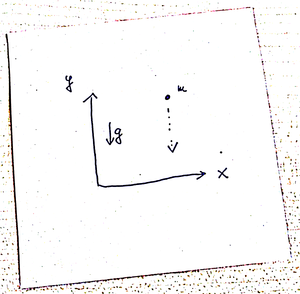
\includegraphics[width=0.4\linewidth]{pics/freefall} 

}

\caption{Free fall of a point mass.}\label{fig:free-fall}
\end{figure}

Here, the laws of the free fall -- a special case of Newton's second law -- applies:

\begin{JHSAYS}
force equals mass times acceleration
\end{JHSAYS}

In 2D, the \(x\), \(y\) coordinates of a point of mass \(m\):

\begin{align*}
m\ddot x &= 0 \\
m\ddot y &= -mg
\end{align*}

where \(g\) is the gravity; see Figure \ref{fig:free-fall}.

\hypertarget{the-pendulum}{%
\subsection*{The Pendulum}\label{the-pendulum}}
\addcontentsline{toc}{subsection}{The Pendulum}

\begin{JHSAYS}
The same point mass attached to a string.
\end{JHSAYS}

\begin{figure}

{\centering 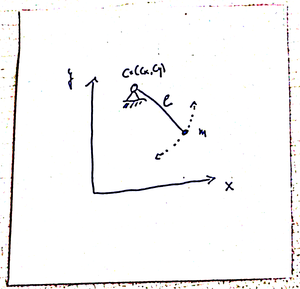
\includegraphics[width=0.4\linewidth]{pics/pendulum} 

}

\caption{A pendulum.}\label{fig:pendulum}
\end{figure}

Again, we have \texttt{force\ =\ mass*acceleration} but also the conditions that the mass moves on a circle:

\[
 (x(t) - c_x)^2 + (y(t) - c_y)^2 = l^2,
\]
where \((c_x, c_y)\) are the coordinates of the center and \(l\) is the length of the string; see Figure \ref{fig:pendulum}.

We use the Lagrangian function to derive the \href{https://en.wikipedia.org/wiki/Lagrangian_mechanics\#Euler\%E2\%80\%93Lagrange_equations_and_Hamilton's_principle}{\emph{Euler-Lagrange equations}} of motion. For the pendulum, we have the kinetic energy
\[
  T = \frac 12 m (\dot x(t)^2 + \dot y(t)^2), 
\]
the potential
\[
U = mgy,
\]
and the constraint
\[
h = (x(t) - c_x)^2 + (y(t) - c_y)^2 - l^2 .
\]

Thus, with \[L:=U-T- \lambda h\] and the requirement that
\[
\frac{d}{dt}(\frac{\partial L}{\partial \dot q}) - \frac{\partial L}{\partial q} = 0
\]
for all of the \emph{generalized coordinates} \(q=x\), \(y\), \(\lambda\),
one obtains a system of equations:

\begin{longtable}[]{@{}lr@{}}
\toprule
Generalized coordinate & Equation\tabularnewline
\midrule
\endhead
\(q \leftarrow x\) & \(m\ddot x(t) + 2 \lambda(t) (x(t) - c_x) = 0\)\tabularnewline
\(q \leftarrow y\) & \(m\ddot y(t) + mgy + 2 \lambda(t) (y(t) - c_y) = 0\)\tabularnewline
\(q \leftarrow \lambda\) & \((x(t) - c_x)^2 + (y(t) - c_y)^2 - l^2 =0\)\tabularnewline
\bottomrule
\end{longtable}

\begin{example}[The Pendulum]
\protect\hypertarget{exm:the-pendulum}{}{\label{exm:the-pendulum} \iffalse (The Pendulum) \fi{} }
After an order reduction via the new variables \(u:=\dot x\) and \(v=\dot y\) the overall system reads

\begin{equation}
\begin{split}
\dot x &= u \\
\dot y &= v \\
m \dot u &= - 2 \lambda (x - c_x) \\ 
m \dot v &= - 2 \lambda (y - c_y) - mgy \\
0&=(x - c_x)^2 + (y - c_y)^2 - l^2, 
\end{split}
\label{eq:pendulum}
\end{equation}

where we have omitted the time dependence.
\end{example}

Equation \eqref{eq:pendulum} is a canonical example for a DAE with combined differential and algebraic equations.

\hypertarget{electrical-circuits}{%
\subsection*{Electrical Circuits}\label{electrical-circuits}}
\addcontentsline{toc}{subsection}{Electrical Circuits}

Another class of DAEs arises from the modelling electrical circuits. We consider the example of \emph{charging a conductor through a resistor} as illustrated in Figure \ref{fig:circuit}.

\begin{figure}

{\centering 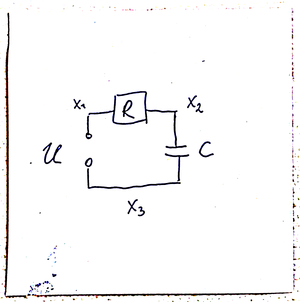
\includegraphics[width=0.4\linewidth]{pics/circuit} 

}

\caption{Electrical circuit with a source, a resistor, and a conductor.}\label{fig:circuit}
\end{figure}

We formulate the problem in terms of the potentials \(x_1\), \(x_2\), \(x_3\), that are assumed to reside in the wires between a source \(U\) and a resistor \(R\), the resistor \(R\) and the capacitor \(C\), and the capacitor and the source.

A model for the circuit is given through the following principles and considerations.

\begin{longtable}[]{@{}lr@{}}
\toprule
\begin{minipage}[b]{0.66\columnwidth}\raggedright
Model principle\strut
\end{minipage} & \begin{minipage}[b]{0.28\columnwidth}\raggedleft
Equation\strut
\end{minipage}\tabularnewline
\midrule
\endhead
\begin{minipage}[t]{0.66\columnwidth}\raggedright
The source defines the difference in the neighboring potentials:\strut
\end{minipage} & \begin{minipage}[t]{0.28\columnwidth}\raggedleft
\(x_1 - x_3 - U = 0\)\strut
\end{minipage}\tabularnewline
\begin{minipage}[t]{0.66\columnwidth}\raggedright
The current \(I_R\) that is induced by the potentials neighboring the resistor is is defined through \emph{Ohm's law}:\strut
\end{minipage} & \begin{minipage}[t]{0.28\columnwidth}\raggedleft
\(I_R = \frac{x_1 - x_2}{R}\)\strut
\end{minipage}\tabularnewline
\begin{minipage}[t]{0.66\columnwidth}\raggedright
The current \(I_C\) that is induced by the potentials neighboring the capacitor is described through:\strut
\end{minipage} & \begin{minipage}[t]{0.28\columnwidth}\raggedleft
\(I_C = C(\dot x_3 - \dot x_2)\)\strut
\end{minipage}\tabularnewline
\begin{minipage}[t]{0.66\columnwidth}\raggedright
Everywhere in the circuit the currents sum up to zero. (This is \emph{Kirchhoff's law}):\strut
\end{minipage} & \begin{minipage}[t]{0.28\columnwidth}\raggedleft
\(I_C + I_R = C(\dot x_3 - \dot x_2)+ \frac{x_1 - x_2}{R}=0\)\strut
\end{minipage}\tabularnewline
\begin{minipage}[t]{0.66\columnwidth}\raggedright
To fix the potential, one can set a ground potential -- here we choose \(x_3\). (note that so far all equations only consider differences in the potential).\strut
\end{minipage} & \begin{minipage}[t]{0.28\columnwidth}\raggedleft
\(x_3 = 0\)\strut
\end{minipage}\tabularnewline
\bottomrule
\end{longtable}

\begin{example}
\protect\hypertarget{exm:the-circuit}{}{\label{exm:the-circuit} }Summing all up, the equations that model the circuit are given as
\begin{equation}
\begin{split}
C(\dot x_3 - \dot x_2) &= - \frac{x_1 - x_2}{R} \\
0  &= x_1 - x_3 - U \\
0 &= x_3. 
\end{split}
\label{eq:circuit}
\end{equation}
\end{example}

\hypertarget{navier-stokes-equations}{%
\subsection*{Navier-Stokes Equations}\label{navier-stokes-equations}}
\addcontentsline{toc}{subsection}{Navier-Stokes Equations}

The Navier-Stokes equations (NSE) are commonly used to model all kind of flows. They describe the evolution of the velocity \(v\) of the fluid and the pressure \(p\) in the fluid. Note that the flow occupies a spatial domain, say in \(\mathbb R^{3}\) so that \(v\) and \(p\) are functions both of the time variable \(t\) and a space variable \(\xi\):

\[
v\colon (t, \xi) \mapsto v(t,\xi)\in \mathbb R^{3} \quad\text{and}\quad  p\colon (t, \xi) \mapsto p(t,\xi)\in \mathbb R.
\]

The NSE:

\begin{align*}
  \frac{\partial v}{\partial t} + (v\otimes \nabla_\xi)v - \Delta_\xi v + \nabla_\xi p &= 0, \\
  \nabla_\xi \cdot v &= 0,
\end{align*}

with \(\otimes\) denoting the outer product and \(\nabla_\xi\) and \(\Delta_\xi\) denoting the gradient and the \emph{Laplace} operator. If we only count the derivatives with respect to time, as postulated in the introduction, the NSE can be seen as an (abstract) DAE.

\begin{JHSAYS}
With \emph{dynamical systems}, we focus on the evolution of time. That's
why the time derivative is relevant for defining DAEs.
\end{JHSAYS}

\hypertarget{automatic-modelling-or-engineers-vs.-mathematicians}{%
\subsection*{\texorpdfstring{Automatic Modelling or \emph{Engineers vs.~Mathematicians}}{Automatic Modelling or Engineers vs.~Mathematicians}}\label{automatic-modelling-or-engineers-vs.-mathematicians}}
\addcontentsline{toc}{subsection}{Automatic Modelling or \emph{Engineers vs.~Mathematicians}}

If a system, say an engine, consists of many interacting processes, it is convenient and common practice to model the dynamics of each particular process and to couple the subprocesses through interface conditions.

This coupling is done through equating quantities so that the overall model will consist of dynamical equations of the subprocesses and algebraic relations at the interfaces -- which makes it a DAE.

In fact, tools like \href{https://www.modelica.org/}{\texttt{modelica}} for automatic modelling of complex processes do exactly this.

\begin{JHSAYS}
The approach of \emph{automatic modelling} is universal and convenient
for engineers. However, the resulting model equations will be DAEs
which, as we will see, pose particular problems in their analytical and
numerical treatment.
\end{JHSAYS}

\hypertarget{why-are-daes-difficult-to-treat}{%
\section{Why are DAEs difficult to treat}\label{why-are-daes-difficult-to-treat}}

Firstly, DAEs do not have the smoothing properties of ODEs, where the solution is one degree smoother than the right hand side. Secondly, the algebraic constraints are essential for the validity of the model. Thus, a numerical approximation may render the model infeasible.

\hypertarget{non-smooth-solutions}{%
\subsection*{Non-smooth Solutions}\label{non-smooth-solutions}}
\addcontentsline{toc}{subsection}{Non-smooth Solutions}

\begin{example}
\protect\hypertarget{exm:nonsmooth-sols}{}{\label{exm:nonsmooth-sols} }Consider the equation

\begin{align*}
    \dot x_1(t) &= x_2(t) \\
        0 & = x_2(t) -g(t)
\end{align*}

where \(g\) can be a nonsmooth function like

\[
    g(t) = 
    \begin{cases} 
        0, \quad\text{if}\quad t < 1 \\
        1, \quad\text{if}\quad t \geq 1 \\
    \end{cases}
\]

In this case the solution part \(x_1=const. + \int_0^tg(s)ds\) will be a smooth function and the solution part \(x_2=g\) will have jumps.
\end{example}

\begin{JHSAYS}
Even worse, the solution of a DAE may depend on derivatives of the right
hand sides.
\end{JHSAYS}

This observation indicates that certain difficulties will arise since

\begin{itemize}
\tightlist
\item
  numerical approximation schemes require smoothness of the solutions
\item
  differentiation is numerically ill-posed unlike numerical integration
\end{itemize}

\hypertarget{numerical-solution-means-approximation}{%
\subsection*{Numerical Solution Means Approximation}\label{numerical-solution-means-approximation}}
\addcontentsline{toc}{subsection}{Numerical Solution Means Approximation}

Imagine the equations \eqref{eq:pendulum} that describe the pendulum are solved approximately. Then, the algebraic constraint will be violated, i.e.~the point mass will leave the circle and the obtained numerical solution becomes infeasible.

Thus, special care has to be taken of the algebraic constraints when the equations of motions are numerically integrated.

\hypertarget{basic-definitions-and-notions}{%
\chapter{Basic Definitions and Notions}\label{basic-definitions-and-notions}}

In a very general form, a DAE can be written as

\begin{equation}
    F(t, x(t), \dot x(t)) = 0
    \label{eq:gendae}
\end{equation}

with \(F\colon \mathbb I \times D_x \times D_{\dot x} \to \mathbb R^m\) and with a time interval \(\mathbb I=[t_0,t_e) \subset \mathbb R\) and state spaces \(D_x\), \(D_{\dot x} \subset \mathbb R^{n}\) and the task to find a function

\begin{equation*}
    x \colon \mathbb I \to \mathbb R^{n}
\end{equation*}

with time derivative \(\dot x \colon \mathbb I \to \mathbb R^{n}\) such that \eqref{eq:gendae} is fulfilled for all \(t\in I\).

A dynamical process that evolves in time needs an initial state. Thus, one can expect a unique solution to the DAEs only if an initial value is prescribed

\begin{equation}
    x(t_0) = x_0 \in \mathbb R^{n}. \label{eq:gendaeiniv} 
\end{equation}

\begin{JHSAYS}
The form of \(F(t, x(t), \dot x(t))\) is a very formal way to write down
a system of differential and algebraic equations. \textbf{X}: Write down
the equations of the previous examples in this form -- i.e.~define
suitable functions \(F\), \(x\), and \(\dot x\).
\end{JHSAYS}

\hypertarget{solution-concept}{%
\section{Solution Concept}\label{solution-concept}}

In order to talk of solutions, we need to define what we understand as a solution.

\begin{definition}
\protect\hypertarget{def:dae-solution}{}{\label{def:dae-solution} }\(\quad\)

\begin{enumerate}
\def\labelenumi{\arabic{enumi}.}
\item
  A function \(x \in \mathcal C^1(\mathbb I, \mathbb R^{n})\) is called a \emph{solution to the DAE} \eqref{eq:gendae}, if \(F(t, x(t), \dot x(t)) = 0\) holds for all \(t\in \mathbb I\).
\item
  A function \(x \in \mathcal C^1(\mathbb I, \mathbb R^{n})\) is called a \emph{solution to the initial value problem} \eqref{eq:gendae} and \eqref{eq:gendaeiniv}, if, furthermore, \(x(t_0)= x_0\) holds.
\item
  An initial condition \eqref{eq:gendaeiniv} is called consistent for the DAE \eqref{eq:gendae}, if there exists at least one solution as defined in 2.
\end{enumerate}
\end{definition}

Some remarks

\begin{itemize}
\tightlist
\item
  The requirement that \(x \in \mathcal C^1\) could be relaxed. Compare Example \ref{exm:nonsmooth-sols}, where certain components of the solution where smoother than others.
\item
  Consistency of initial values is a major issue in the treatment of DAEs. See the pendulum\ldots{}
\end{itemize}

\hypertarget{initial-conditions-and-consistency}{%
\section{Initial Conditions and Consistency}\label{initial-conditions-and-consistency}}

We consider again the equations of motions of the pendulum (Example \ref{exm:the-pendulum})

\begin{align*}
    \dot x(t) &= u(t) \\
    \dot y(t) &= v(t) \\
    m \dot u(t) &= - 2 \lambda(t) (x(t) - c_x) \\ 
    m \dot v(t) &= - 2 \lambda(t) (y(t) - c_y) - mgy(t)
\end{align*}

with the constraint

\begin{equation}
    0=(x(t) - c_x)^2 + (y(t) - c_y)^2 - l^2. \label{eq:pendulum-rvst-cnstrt}
\end{equation}

To use this model to predict the time evolution of the system, a starting point needs to be known, say for \(t=0\). This means initial positions and initial velocities:

\[
\begin{bmatrix} 
x(0) \\ y(0)
\end{bmatrix}
=
\begin{bmatrix} 
    x_0 \\ y_0
\end{bmatrix}
\quad\text{and}\quad
\begin{bmatrix} 
u(0) \\ v(0)
\end{bmatrix}
=
\begin{bmatrix} 
    u_0 \\ v_0
\end{bmatrix}.
\]

The constraint \eqref{eq:pendulum-rvst-cnstrt} needs to be fulfilled at all times and also at \(t=0\), which gives the constraint for the initial positions:

\begin{equation*}
    (x_0 - c_x)^2 + (y_0 - c_y)^2 - l^2=0.
\end{equation*}

Moreover, if a constraint \(h(x(t), y(t))=0\) holds for all \(t\), then, necessarily, \(\frac{d}{dt}h=0\). For the pendulum this means that

\begin{equation}
    2(x(t) - c_x)u(t) + 2(y(t) - c_y)v(t) = 0 \label{eq:pendulum-rvst-cnstrt-ddt}
\end{equation}

must hold for all \(t\) and in particular at \(t=0\) which gives constraints on the initial velocities \(u_0\) and \(v_0\):

\begin{equation*}
    2(x_0 - c_x)u_0 + 2(y_0 - c_y)v_0 = 0.
\end{equation*}

Some remarks on consistency, constraints, and derivations:

\begin{itemize}
\tightlist
\item
  The so-called \emph{consistency conditions} on \((x_0, y_0, u_0, v_0)\) have the physical interpretation that the initial positions lie on the prescribed circle and that the velocities are tangent to this circle.
\item
  One can show that the variable \(\lambda\) is completely defined in terms of \(x\) and \(y\) and their derivatives. Thus, in the formulation \eqref{eq:pendulum}, both in the analysis and in the numerical treatment, there is no need for an initial value for \(\lambda\). However, as we will see, DAEs can be reformulated as ODEs through differentiation and substitutions. In such an ODE formulation, a necessary initial condition for \(\lambda\) will have to fulfill similar consistency conditions as \((x_0, y_0, u_0, v_0)\).
\end{itemize}

Condition \eqref{eq:pendulum-rvst-cnstrt-ddt} is an example for a \emph{hidden-constraint} -- an algebraic constraint to the system that is not explicit in the original formulation. In theory, condition \eqref{eq:pendulum-rvst-cnstrt} can be replaced by \eqref{eq:pendulum-rvst-cnstrt-ddt}. Moreover, through differentiation and elimination of constraints, a DAE can be brought into the form of an ODE: in the case of the circuit of Example \ref{exm:the-circuit} one only needs to replace the constraints by their derivatives:

\begin{equation}
\begin{split}
C(\dot x_3 - \dot x_2) &= - \frac{x_1 - x_2}{R} \\
\dot x_1 - \dot x_3 &= \dot U \\
\dot x_3 &= 0. 
\end{split}
\label{eq:circuit-ddt}
\end{equation}

Note that \eqref{eq:circuit-ddt} can be written as \(B\dot x = Ax + f\) with an invertible matrix \(B\) and, thus, is an ODE.

For an ODE there is no constraint on the initial values. However, a solution to \eqref{eq:circuit-ddt} only solves the original DAE \eqref{eq:circuit}, if the initial values are consistent with the DAE. In this case, this means \(x_3(t_0)=0\) and \(x_1(t_0) - x_3(t_0) = U(t_0)\).

\hypertarget{additional-remarks}{%
\section{Additional Remarks}\label{additional-remarks}}

\begin{itemize}
\item
  It just took a single derivation to turn the circuit model into an ODE \eqref{eq:circuit-ddt}. For the \emph{pendulum} this wouldn't be that easy.
\item
  The extend of how much algebraic and differential parts are intertwined is measured by \emph{indices} which is \textbf{the classifier} for DAEs.
\item
  There are many indices. We will learn about some of the concepts. But first we will introduce some more theory.
\end{itemize}

\begin{JHSAYS}
A low index means that differential and algebraic parts are relatively
well separated. (The circuit example is of \emph{index 1}). A high index
means that the structure is more involved. (The pendulum is of
\emph{index 3}).
\end{JHSAYS}

\hypertarget{III}{%
\chapter{Linear DAEs with Constant Coefficients}\label{III}}

\hypertarget{basic-notions-and-definitions}{%
\section{Basic Notions and Definitions}\label{basic-notions-and-definitions}}

Consider the DAE in the form
\begin{equation}
E \dot x (t) = Ax(t) + f(t), \label{eq:gen-lin-cc-dae}
\end{equation}
where \(E\), \(A\in \mathbb R^{m,n}\) and \(f\in \mathcal C(\mathbb I, \mathbb R^m)\) with, possibly, an initial condition
\begin{equation}
x(t_0) = x_0 \in \mathbb R^{n}. \label{eq:gen-lin-cc-dae-inic}
\end{equation}

\begin{JHSAYS}
For utmost generality, we consider the case that \(m\neq n\), i.e.~the
number of equations does not meet the number of unknowns, but we will
turn to the square case of \(m=n\) soon.
\end{JHSAYS}

\hypertarget{scalings-and-state-transformations}{%
\subsection{Scalings and State Transformations}\label{scalings-and-state-transformations}}

One can confirm that if \(x\) is a solution to \eqref{eq:gen-lin-cc-dae} and \(P\in \mathbb R^{n,n}\) is invertible, then \(x\) is a solution to
\begin{equation*}
PE \dot x (t) = PAx(t) + Pf(t).
\end{equation*}

\begin{JHSAYS}
This is a scaling of the equations.
\end{JHSAYS}

Similarly, if \(Q\in \mathbb R^{n,n}\) is invertible, then \(\tilde x := Q^{-1}x\) solves

\begin{equation*}
E Q \dot {\tilde x} (t) = AQ \tilde x(t) + f(t).
\end{equation*}

\begin{JHSAYS}
This is a state transformation of the system.
\end{JHSAYS}

Thus, when talking of solvability of \eqref{eq:gen-lin-cc-dae}, one may equivalently consider any regular \(Q\in \mathbb R^{m,m}\), \(P\in \mathbb R^{m,m}\) and the scaled and transformed system
\begin{equation}
\tilde E \dot{\tilde x}(t) = \tilde A \tilde x (t) + \tilde f(t), \quad \tilde x(0) = Q^{-1}x_0,
\end{equation}
where \(\tilde E = PEQ\), \(\tilde A = PAQ\), \(\tilde f = Pf\), and \(x=Q\tilde x\).

To characterize all scalings and state transformations, we define these operations as relations of matrix pairs:

\hypertarget{strong-equivalence-and-canonical-forms}{%
\subsection{Strong Equivalence and Canonical Forms}\label{strong-equivalence-and-canonical-forms}}

\begin{definition}
\protect\hypertarget{def:matrix-pair-equivalent}{}{\label{def:matrix-pair-equivalent} }Two pairs of matrices \((E_1, A_1)\) and \((E_2, A_2)\), with \(E_1\), \(A_1\), \(E_2\), \(A_2 \in \mathbb R^{m,n}\), are called \emph{strongly equivalent}, if there exist regular matrices \(P\in \mathbb R^{m,m}\), \(Q\in \mathbb R^{n,n}\) such that
\begin{equation*}
E_2 = PE_1Q, \quad A_2 = PA_1Q.
\end{equation*}
In this case, we write
\[(E_1, A_1) \sim (E_2, A_2).\]
\end{definition}

\begin{lemma}
\protect\hypertarget{lem:strong-equivalence-RSI}{}{\label{lem:strong-equivalence-RSI} }The relation \(\sim\) defined in Definition \ref{def:matrix-pair-equivalent} defines an equivalence relation\footnote{Equivalence relation -- \textbf{RST}. \textbf{R}eflexive: \(A\sim A\). \textbf{S}ymmetric: \(A\sim B\), then \(B\sim A\). \textbf{T}ransitive: \(A\sim B\) and \(B\sim C\), then \(A\sim C\).}.
\end{lemma}
\begin{proof}
\iffalse{} {Proof. } \fi{}Exercise.
\end{proof}

For a given equivalence relation on a set, one can define \emph{equivalence classes} by considering all members that are equivalent to each other as basically the same. And for each class one may choose a representative, preferably in \emph{canonical form}, i.e.~a form that, e.g.,

\begin{enumerate}
\def\labelenumi{\arabic{enumi}.}
\tightlist
\item
  comes with an simple or characteristic representation and
\item
  that allows for easy determination or analysis of quantities of interest.
\end{enumerate}

\begin{JHSAYS}
There can be infinitely many canonical forms. For our purposes and for
the \emph{strong equivalence} of matrix pairs, we will use the
\emph{Kronecker Canonical Form}.
\end{JHSAYS}

\begin{theorem}
\protect\hypertarget{thm:kcf}{}{\label{thm:kcf} }
Let \(E\), \(A \in \mathbb C^{m,n}\). Then there exist nonsingular matrices \(P\in \mathbb C^{m,m}\), \(Q\in \mathbb C^{n,n}\) such that for all \(\lambda \in \mathbb C\)
\begin{equation*}
P(\lambda E -A)Q = 
\begin{bmatrix}
\mathcal L_{\epsilon_1} \\
& \ddots \\
&& \mathcal L_{\epsilon_p} \\
&&& \mathcal M_{\eta_1} \\
&&&& \ddots \\
&&&&& \mathcal M_{\eta_q} \\
&&&&&& \mathcal J_{\rho_1} \\
&&&&&&& \ddots \\
&&&&&&&& \mathcal J_{\rho_r} \\
&&&&&&&&& \mathcal N_{\sigma_1} \\
&&&&&&&&&& \ddots \\
&&&&&&&&&&& \mathcal N_{\sigma_s}
\end{bmatrix}
\end{equation*}
Where the block entries are as follows:

\begin{enumerate}
\def\labelenumi{\arabic{enumi}.}
\tightlist
\item
  Every entry \(\mathcal L_{\epsilon_j}\) is bidiagonal of size \(\epsilon_j\times (\epsilon_j +1)\), \(\epsilon_j \in \mathbb N \cup \{0\}\) of the form
  \begin{equation*}
  \lambda 
  \begin{bmatrix}
  0 & 1  \\
  & \ddots & \ddots \\
  && 0 & 1
  \end{bmatrix}
  -
  \begin{bmatrix}
  1 & 0  \\
  & \ddots & \ddots \\
  && 1 & 0
  \end{bmatrix}
  \end{equation*}
\item
  Every entry \(\mathcal M_{\eta_j}\) is bidiagonal of size \((\eta_j+1)\times \eta_j\), \(\eta_j \in \mathbb N \cup \{0\}\) of the form
  \begin{equation*}
  \lambda 
  \begin{bmatrix}
  1  \\
  0 & \ddots \\
  & \ddots & 1 \\
  && 0 
  \end{bmatrix}
  -
  \begin{bmatrix}
  0  \\
  1 & \ddots \\
  & \ddots & 0 \\
  && 1 
  \end{bmatrix}
  \end{equation*}
\item
  Every entry \(\mathcal J_{\rho_j}\) is a Jordan block of size \(\rho_j\times \rho_j\), \(\rho_j \in \mathbb N \setminus \{0\}\), \(\lambda_j \in \mathbb C\) of the form
  \begin{equation*}
  \lambda 
  \begin{bmatrix}
  1  \\
  & \ddots \\
  &&\ddots  \\
  &&& 1 
  \end{bmatrix}
  -
  \begin{bmatrix}
  \lambda_j & 1 \\
  & \ddots & \ddots \\
  &&& 1 \\
  &&& \lambda_j 
  \end{bmatrix}
  \end{equation*}
\item
  Every entry \(\mathcal N_{\sigma_j}\) is a nilpotent block of size \(\sigma_j\times \sigma_j\), \(\sigma_j \in \mathbb N \setminus \{0\}\), of the form
  \begin{equation*}
  \lambda 
  \begin{bmatrix}
  0 &1\\
  & \ddots & \ddots \\
  &&& 1  \\
  &&& 0 
  \end{bmatrix}
  -
  \begin{bmatrix}
  1 \\
  & \ddots  \\
  &&&  \\
  &&&& 1 
  \end{bmatrix}
  \end{equation*}
\end{enumerate}

The \emph{Kronecker Canonical Form} is uniquely defined up to permutations of the blocks.
\end{theorem}

\begin{proof}
\iffalse{} {Proof. } \fi{}Very technical. Can be found, e.g., in the book: Gantmacher (1959) \emph{The Theory of Matrices II}.
\end{proof}

Algorithm for computations exist\footnote{Paul v. Dooren \href{https://perso.uclouvain.be/paul.vandooren/publications/VDooren79.pdf}{The Computation of Kronecker's Canonical Form of a Singular Pencil}} but the computation is notoriously ill posed.

\hypertarget{regularity-and-solvability}{%
\section{Regularity and Solvability}\label{regularity-and-solvability}}

In what follows we will consider the regular case with, among others, \(E\) and \(A\) as square matrices.

\begin{JHSAYS}
Like for solving general equation systems, one can expect well posedness
for the case that the numbers of equations equals the number of
unknowns. Here \emph{squareness} of the system is a necessary condition.
For sufficiency one further needs that there are no redundant equations
or incompatible equations. This is encoded in the \emph{regularity}.
\end{JHSAYS}

\begin{definition}
\protect\hypertarget{def:regularity}{}{\label{def:regularity} }Let \(E\), \(A \in \mathbb C^{n,n}\). The matrix pair \((E, A)\) is called \emph{regular}, if the \emph{characteristic polynomial} \(p\), defined via
\[
p(\lambda) = \det (\lambda E- A),
\]
is not identically zero. If such a matrix pair is not regular, it is called \emph{singular}.
\end{definition}

\begin{JHSAYS}
\emph{Is not identically zero} means that there exists a \(\lambda_0\)
such that \(p(\lambda_0)=\det (\lambda_0 E - A) \neq 0\),
i.e.~\(\lambda_0 E - A\) is invertible.
\end{JHSAYS}

\begin{JHSAYS}
Since a characteristic polynomial has but a finite numbers of roots
(unless it is the \emph{zero polynomial}), \emph{is not identically
zero} means that \(p(\lambda) \neq 0\) for all but a few \(\lambda\).
\end{JHSAYS}

Next we show, that \emph{regularity} is invariant under \emph{strong equivalence}. This is needed, since we will translate regularity of \((E,A)\) to regularity of the associated DAE and we need to ensure that regular scalings and state transformations do not affect regularity.

\begin{lemma}
\protect\hypertarget{lem:invariance-regularity}{}{\label{lem:invariance-regularity} }Let \(E\), \(A \in \mathbb C^{n,n}\). If \((E, A)\) is strongly equivalent to a regular matrix pair, then \((E, A)\) is regular.
\end{lemma}

\begin{proof}
\iffalse{} {Proof. } \fi{}Let \(E_1\), \(A_1 \in \mathbb C^{n, n}\) be similar to \((E, A)\). By definition, there exist invertible \(P\), \(Q\in \mathbb C^{n,n}\) such that \(\lambda E - A = P(\lambda E_1 -A_1)Q\) for all \(\lambda\). Thus,
\[
\det (\lambda E - A) = \det P \det (\lambda E_1 - A_1) \det Q
\]
is not identically zero, since \(\det Q\) and \(\det P\) are not zero and \(\det (\lambda E_1 - A_1)\) is not the zero polynomial.
\end{proof}

With that we can derive a \emph{canonical form} for \emph{strongly equivalent} matrix pairs.

\begin{theorem}
\protect\hypertarget{thm:weierstrass-cf}{}{\label{thm:weierstrass-cf} }Let \(E\), \(A \in \mathbb C^{n,n}\) and \((E,A)\) be regular. Then
\begin{equation}
(E, A) \sim 
\left (
\begin{bmatrix}
I_{n_1} \\
& N
\end{bmatrix}
,
\begin{bmatrix}
J \\
& I_{n_2}
\end{bmatrix}
\right ),
\label{eq:weierstrass-cf}
\end{equation}

\begin{itemize}
\tightlist
\item
  where \(n_1\), \(n_2 \in \mathbb N\) such that \(n=n_1+n_2\),
\item
  where \(I_{n_1}\) and \(I_{n_2}\) denote the identity matrices of size \(n_1\times n_1\) and \(n_2\times n_2\), respectively,
\item
  where \(J\in \mathbb C^{n_1,n_1}\) is in \emph{Jordan canonical form},
\item
  and where \(N \in \mathbb C^{n_2,n_2}\) is a \protect\hyperlink{def:nilpotent-matrix}{\emph{nilpotent} matrix}.
\item
  Moreover, it is allowed that the one or the other block is not present, i.e., \(n_1\) or \(n_2\) can be zero.
\end{itemize}
\end{theorem}

\begin{proof}
\iffalse{} {Proof. } \fi{}To be provided.
\end{proof}

Recall that the \emph{Jordan canonical form} can be achieved for any square matrix \(M\in \mathbb C\) by a similarity transformation.

\begin{definition}[Nilpotent Matrix]
\protect\hypertarget{def:nilpotent-matrix}{}{\label{def:nilpotent-matrix} \iffalse (Nilpotent Matrix) \fi{} }A matrix \(M\in \mathbb C^{n,n}\) is called \emph{nilpotent}, if there is an integer \(k\) such that \(M^k=0\). The smallest such integer \emph{index}, i.e.~that \(\nu \in \mathbb N\) such that \(N^\nu=0\) whereas \(N^{\nu-1} \neq 0\) is called the \emph{index of nilpotency} of \(M\).
\end{definition}

\begin{JHSAYS}
With the convention that \(\mathbf 0^0=I\), the zero matrix
\(\mathbf 0 \in \mathbb R^{n,n}\) is of (nilpotency) index 1.
\end{JHSAYS}

The relation of solvability and regularity of DAEs becomes evident in the canonical form of Theorem \ref{thm:weierstrass-cf}. In fact, it states that through regular scalings and state transforms, any DAE with

\[
E\dot x(t) =  A x(t) + f(t)
\]

with \((E,A)\) regular can be transformed and split into
\begin{equation}
\dot x_1(t) = x_1(t) + f_1(t) \label{eq:reg-dae-wcf-diffpart}
\end{equation}
and
\begin{equation}
N \dot x_2(t) = x_2(t) + f_2(t) \label{eq:reg-dae-wcf-algpart},
\end{equation}

i.e

\begin{itemize}
\tightlist
\item
  into an \textbf{ODE} \eqref{eq:reg-dae-wcf-diffpart} that already is in \emph{Jordan canonical form}
\item
  and a separated(!) \textbf{DAE} \eqref{eq:reg-dae-wcf-algpart} of a particular type.
\end{itemize}

Since linear ODEs always have a unique solution for any initial value, solvability of a general linear DAE with constant, regular coefficients will be completely defined by solvability of the special DAE part \eqref{eq:reg-dae-wcf-algpart}.

\hypertarget{solution-to-the-n-dae-regularity-and-index-of-a-matrix-pair}{%
\section{\texorpdfstring{Solution to the \emph{N-DAE}, Regularity, and Index of a Matrix Pair}{Solution to the N-DAE, Regularity, and Index of a Matrix Pair}}\label{solution-to-the-n-dae-regularity-and-index-of-a-matrix-pair}}

In what follows we will consider the special DAE
\begin{equation}
N \dot x(t) = x(t) + f(t) \label{eq:ndae}
\end{equation}
with \(N \in \mathbb R^{n,n}\) nilpotent with \(\nu\) being the \protect\hyperlink{def:nilpotent-matrix}{index of nilpotency}.
For this DAE there is an explicit solution formula:

\begin{lemma}
\protect\hypertarget{lem:ndae-explicit-solution}{}{\label{lem:ndae-explicit-solution} }Consider \eqref{eq:ndae}. If \(f \in \mathcal C^\nu(\mathcal I, \mathbb R^{n})\), \(n\geq 1\), where \(\nu\) is the index of nilpotency of \(N\), then \eqref{eq:ndae} has a unique solution given as
\begin{equation}
x(t) = - \sum_{i=0}^{\nu-1}N^if^{(i)}(t), \label{eq:iii-ndae-exp-solution}
\end{equation}
where \(f^{(i)}\) denotes the \(i\)-th derivative of \(f\).
\end{lemma}

\begin{proof}
\iffalse{} {Proof. } \fi{}There are a few ways to prove the explicit form \eqref{eq:iii-ndae-exp-solution}

\begin{enumerate}
\def\labelenumi{\arabic{enumi}.}
\item
  Bring \(N\) into Jordan canonical form and prove the formula for the Jordan blocks of arbitrary size by induction.
\item
  Write \eqref{eq:ndae} as \[(N\frac{d}{dt}-I)x = f\] and show that\footnote{See the proof of Lemma 2.8 in \emph{Kunkel/Mehrmann}} \[(N\frac{d}{dt}-I)^{-1} = - \sum_{i=0}^{\nu-1}N^i\frac{d^i}{dt^i}\].
\item
  We take the direct approach as it can be found in the book by Dai\footnote{Dai (1989): \emph{Singular Control Systems}}:
\end{enumerate}

Firstly, we observe that
\[
x = N\dot x - f.
\]
Secondly, that (having multiplied by \(N\) and differentiated once)
\[
N\dot x = N^2 \ddot x - N \dot f.
\]
And, finally, that (having muliplied \(k\)-times by \(N\) and differentiated \(k\)-times)
\[
N^k\dot x^{(k)} = N^{k+1} \dot x^{(k+1)} - N^k \dot f^{(k)}.
\]
If one successively replaces \(N^kx^{(k)}=N^{k+1}x^{(k+1)}-N^kf^{(k)}\), \(k=1,2,...,\nu-1\) in
\[
x=N\dot x -f = N^2\ddot x - N\dot f -f = \dots = N^\nu x^{(\nu)} - \sum_{i=0}^{\nu-1} N^if^{(i)},
\]
with \(N^\nu=0\), one arrives at formula \eqref{eq:iii-ndae-exp-solution}.

Since this construction holds for any solution, uniqueness is guaranteed too.
\end{proof}

\begin{JHSAYS}
We make three important observations here.
\end{JHSAYS}

\begin{enumerate}
\def\labelenumi{\arabic{enumi}.}
\item
  The solution \(x\) to \eqref{eq:ndae} is uniquely defined without specifying a value at \(t_0\). Vice versa, an initial value \(x_0\) is consistent if, and only if,
  \[
  x_0 = - \sum_{i=0}^{\nu-1}N^if^{(i)}(t_0)
  \]
\item
  The definition of the solution \(x\) requires \(f\) to be \(\nu-1\)-times differentiable. In order to be a solution according to Definition \ref{def:dae-solution}, the function \(x\) itself has to be differentiable too. Hence the requirement \(f \in \mathcal C^\nu(\mathcal I, \mathbb R^{n})\).
\item
  The index of nilpotency of \(N\) defines the necessary smoothness of the right hand side.
\end{enumerate}

\begin{JHSAYS}
The index of nilpotency in the \(N\) part of the
\protect\hyperlink{eq:weierstrass-cf}{Weierstrass canonical form} is
characteristic for a matrix pair and defines an \emph{index} of the
associated DAE.
\end{JHSAYS}

\begin{definition}
\protect\hypertarget{def:matrix-pair-index}{}{\label{def:matrix-pair-index} }Consider a regular matrix pair \((E, A)\) and its Weierstrass canonical form, i.e.
\[
(E, A) \sim 
\left (
\begin{bmatrix}
I_{n_1} \\
& N
\end{bmatrix}
,
\begin{bmatrix}
J \\
& I_{n_2}
\end{bmatrix}
\right ).
\]
The index \(\nu\) of nilpotency of \(N\) is called the index of the matrix pair \((E, A)\) and we write \(\nu = \operatorname{ind}(E, A)\). If \(N\) is not present, then we set \(\operatorname{ind}(E,A)=0\).
\end{definition}

\begin{JHSAYS}
Furthermore, for a nilpotent matrix \(N\), we will occasionally use the
notion \(\nu=\operatorname{ind}(N,I)\) to refer to its index of nilpotency.
\textbf{X}: Is this OK, i.e.~consistent?
\end{JHSAYS}

To be on the safe side and to learn how to handle block structured matrices in the analysis, we confirm that this definition of the index is well-posed, i.e.~for any regular matrix \((E,A)\) there is a unique index \(\nu\).

\begin{JHSAYS}
If one considers the Weierstrass canonical form as a special case of the
\protect\hyperlink{thm:kcf}{Kronecker canonical form}, then the
statement that \emph{the canonical form is well-posed up to permutations
in the order of the blocks} already implies that the index is well
defined (since it only depends on the size of the largest nilpotent
block but not in which order it appears).
\end{JHSAYS}

\begin{lemma}
\protect\hypertarget{lem:kronecker-index-well-defined}{}{\label{lem:kronecker-index-well-defined} }Suppose that the regular matrix pair \((E, A)\), \(E\), \(A\in \mathbb R^{n,n}\) has the two canonical forms
\[
(E, A) \sim 
\left (
\begin{bmatrix}
I_{d_1} \\
& N_1
\end{bmatrix}
,
\begin{bmatrix}
J_1 \\
& I_{n-d_1}
\end{bmatrix}
\right )
\sim 
\left (
\begin{bmatrix}
I_{d_2} \\
& N_2
\end{bmatrix}
,
\begin{bmatrix}
J_2 \\
& I_{n-d_2}
\end{bmatrix}
\right ),
\]
where \(d_1\), \(d_2\) are the size of the Jordan blocks \(J_1\), \(J_2\), respectively. Then \(d_1=d_2=:d\) and the indices of nilpotency of the nilpotent blocks coincide, i.e.~\(\operatorname{ind}(N_1, I_{n-d}) = \operatorname{ind}(N_2, I_{n-d})\).
\end{lemma}
\begin{proof}
\iffalse{} {Proof. } \fi{}To show that \(d_1=d_2\), without loss of generality, we can assume that \(N_i\) are in Jordan form too. This, in particular, means that they are upper triangular with zeros on the diagonal. (If this was not the case, we can use \(N_i = T^{-1}\tilde N_i T\) in the arguments below).

Then, we have that the characteristic polynomials
\[
\det (\lambda E - A) = \det (\lambda N_i-I_{n-d_i})\det (\lambda I_{d_i} - J_i) = (-1)^{n-d_i}\det (\lambda I_{d_i} - J_i)
\]
are polynomials of degree \(d_i\), \(i=1,2\).

Since the characteristic polynomials of strongly equivalent matrix pairs only differ by a constant factor (see the proof of Lemma \ref{lem:invariance-regularity}), this implies that \(d_1=d_2\).

Now we show, that the indices of nilpotency of \(N_1\) and \(N_2\) coincide. If the \(N\)-blocks weren't present, there would be nothing to show. So let's assume that they are there.

Let now be \(P\), \(Q \in \mathbb R^{n,n}\) that invertible matrices that realize the strong equivalence of the canonical forms, i.e.
\begin{equation}
\label{eq:equiv-wcf-i}
\begin{bmatrix}
P_{11} & P_{12} \\
P_{21} & P_{22}
\end{bmatrix}
\begin{bmatrix}
I \\
& N_2
\end{bmatrix}
=
\begin{bmatrix}
I \\
& N_1 
\end{bmatrix}
\begin{bmatrix}
Q_{11} & Q_{12} \\
Q_{21} & Q_{22}
\end{bmatrix}
\end{equation}
and
\begin{equation}
\label{eq:equiv-wcf-ii}
\begin{bmatrix}
P_{11} & P_{12} \\
P_{21} & P_{22}
\end{bmatrix}
\begin{bmatrix}
J_2 \\
& I 
\end{bmatrix}
=
\begin{bmatrix}
J_1 \\
& I 
\end{bmatrix}
\begin{bmatrix}
Q_{11} & Q_{12} \\
Q_{21} & Q_{22}
\end{bmatrix},
\end{equation}
where \(P\) and \(Q\) have been partitioned in line with the canonical forms.

Taking the blockwise matrix product and equating the blocks separately, the following relations are obtained:

\begin{longtable}[]{@{}lcccc@{}}
\toprule
\begin{minipage}[b]{0.11\columnwidth}\raggedright
Block:\strut
\end{minipage} & \begin{minipage}[b]{0.19\columnwidth}\centering
(1,1)\strut
\end{minipage} & \begin{minipage}[b]{0.19\columnwidth}\centering
(1,2)\strut
\end{minipage} & \begin{minipage}[b]{0.19\columnwidth}\centering
(2,1)\strut
\end{minipage} & \begin{minipage}[b]{0.19\columnwidth}\centering
(2,2)\strut
\end{minipage}\tabularnewline
\midrule
\endhead
\begin{minipage}[t]{0.11\columnwidth}\raggedright
\eqref{eq:equiv-wcf-i}:\strut
\end{minipage} & \begin{minipage}[t]{0.19\columnwidth}\centering
\(P_{11}=Q_{11}\)\strut
\end{minipage} & \begin{minipage}[t]{0.19\columnwidth}\centering
\(P_{12}N_2=Q_{12}\)\strut
\end{minipage} & \begin{minipage}[t]{0.19\columnwidth}\centering
\(P_{21}=N_1Q_{21}\)\strut
\end{minipage} & \begin{minipage}[t]{0.19\columnwidth}\centering
\(P_{22}N_2=N_1Q_{22}\)\strut
\end{minipage}\tabularnewline
\begin{minipage}[t]{0.11\columnwidth}\raggedright
\eqref{eq:equiv-wcf-ii}:\strut
\end{minipage} & \begin{minipage}[t]{0.19\columnwidth}\centering
\(P_{11}J_2=J_1Q_{11}\)\strut
\end{minipage} & \begin{minipage}[t]{0.19\columnwidth}\centering
\(P_{12}=J_1Q_{12}\)\strut
\end{minipage} & \begin{minipage}[t]{0.19\columnwidth}\centering
\(P_{21}J_2=Q_{21}\)\strut
\end{minipage} & \begin{minipage}[t]{0.19\columnwidth}\centering
\(P_{22}=Q_{22}\)\strut
\end{minipage}\tabularnewline
\bottomrule
\end{longtable}

If we combine the \textbf{(2,1)} blocks, we obtain that
\[
P_{21}=N_1Q_{21}=N_1P_{21}J_2=N_1^2P_{21}J_2^2=N_1^3P_{21}J_2^3=\dotsc=0
\]
since \(N_1\) is nilpotent.

Since \(P\) is invertible and, because of \(P_{21}=0\), block upper triangular, the blocks on the diagonals \(P_{11}\) and \(P_{22}\) must be invertible. With \(Q_{22}=P_{22}\) the \textbf{(2,2)} block of \eqref{eq:equiv-wcf-i} implies that
\[
N_2 = P_{22}^{-1}N_1P_{22}
\]
and, further,
\[
N_2^k = P_{22}^{-1}N_1^kP_{22}
\]
for all \(k\in\mathbb N\). So that a power \(N_2^k=0\) if, and only if, \(N_1^k=0\). Consequently, the indices of nilpotency of \(N_1\) and \(N_2\) coincide.
\end{proof}

\hypertarget{III-ex-sols}{%
\section{Existence of Solutions}\label{III-ex-sols}}

\begin{JHSAYS}
We can now summarize all results and considerations in a theorem.
\end{JHSAYS}

\begin{theorem}
\protect\hypertarget{thm:regularity-means-solvability}{}{\label{thm:regularity-means-solvability} }
Consider the DAE \eqref{eq:gen-lin-cc-dae} with initial condition \eqref{eq:gen-lin-cc-dae-inic},
\[
E \dot x (t) = Ax(t) + f(t), \quad x(t_0) = x_0 \in \mathbb R^{n}.
\]
Let the pair \((E, A)\) be \protect\hyperlink{lem:regularity}{regular} and consider the strongly equivalent DAE
\[
\tilde E \dot {\tilde x} (t) = \tilde A\tilde x(t) + \tilde f(t), \quad \tilde x(t_0) = \tilde x_0 \in \mathbb R^{n}.
\]
with \((\tilde E,\tilde A)\) in Weierstrass canonical form, i.e.
\[
\tilde E = 
\begin{bmatrix}
I & 0 \\  0 &N 
\end{bmatrix}, 
\quad 
\tilde A = 
\begin{bmatrix}
J & 0 \\  0 &I 
\end{bmatrix}, 
\]
and consider the conforming splitting of the transformed variables
\[
\tilde x = 
\begin{bmatrix}
\tilde x_1 \\ \tilde x_2
\end{bmatrix},
\quad
\tilde x_0 = 
\begin{bmatrix}
\tilde x_{0,1} \\ \tilde x_{0,2}
\end{bmatrix}.
\]
Furthermore, let \(\nu\) be the index of the matrix pair \((E,A)\).

If \(f\in \mathcal C^\nu(\mathcal I,\mathbb C^{n})\), then

\begin{enumerate}
\def\labelenumi{\arabic{enumi}.}
\item
  The differential algebraic equation \eqref{eq:gen-lin-cc-dae} is solvable.
\item
  The initial condition \(x_0\) in \eqref{eq:gen-lin-cc-dae-inic} is consistent if, and only if, for the transformed initial condition \(\tilde x_0\) it holds that
  \[
    \tilde x_{2,0} = - \sum_{i=0}^{\nu-1}N^i\tilde f^{(i)}(t_0)
  \]
  In particular, a consistent initial condition to \eqref{eq:gen-lin-cc-dae} exists.
\item
  Every initial value problem \eqref{eq:gen-lin-cc-dae}--\eqref{eq:gen-lin-cc-dae-inic} with a consistent initial condition is uniquely solvable.
\end{enumerate}
\end{theorem}

\begin{proof}
\iffalse{} {Proof. } \fi{}A summary of the preceding results.
\end{proof}

From Theorem \ref{thm:regularity-means-solvability} it follows that the regularity of the matrix pair \((E, A)\) implies the existence of a unique solution to the DAE \eqref{eq:gen-lin-cc-dae} with an initial condition \eqref{eq:gen-lin-cc-dae-inic} provided that the initial condition is consistent.

\begin{JHSAYS}
The negation of this statement is a bit diffuse because there are
several things that \emph{can go wrong} if the DAE is not regular.
Depending on the irregularity there might be infinite many solutions to
the initial value problem or no solutions at all to the DAE (even
without the initial condition).
\end{JHSAYS}

The following theorem covers the case of singular or non-square matrix pairs.

\begin{theorem}[Thm. 2.14 in *Kunkel/Mehrmann*]
\protect\hypertarget{thm:unnamed-chunk-22}{}{\label{thm:unnamed-chunk-22} \iffalse (Thm. 2.14 in \emph{Kunkel/Mehrmann}) \fi{} }Let \(E\), \(A\in \mathbb C^{m,n}\).

\begin{enumerate}
\def\labelenumi{\arabic{enumi}.}
\item
  If \(\operatorname{rank}(\lambda E -A) < n\) for all \(\lambda \in \mathbb C\), then the \emph{homogeneous} initial value problem
  \[ 
  E\dot x(t) = Ax(t), \quad x(t_0) = 0, 
  \]
  has a nontrivial solution.
\item
  If \(\operatorname{rank}(\lambda E -A) < m\) for all \(\lambda\in \mathbb C\), then there exist arbitrarily smooth inhomogeneities \(f\) for which the DAE \eqref{eq:gen-lin-cc-dae}
  \[ 
  E\dot x(t) = Ax(t)+f(t),
  \]
  is not solvable.
\end{enumerate}
\end{theorem}

\begin{proof}
\iffalse{} {Proof. } \fi{}The proof is given for Theorem 2.14 in \emph{Kunkel/Mehrmann} with, however, the second claim being formulated slightly differently. To reduce our formulation to \emph{theirs}, one may identify that columns of \(\lambda E - A\) that achieve the maximal rank and split off the redundant columns, e.g., the parts of \(x\) associated with them.
\end{proof}

Note that a nontrivial solution to the \emph{homogeneous} problem, means that existence of \textbf{a} solution implies \textbf{infinitely many} solutions to the initial value problem. In fact, if \(x_h\) is the solution to the homogeneous problem and \(x_p\) a solution\footnote{A so-called particular solution. Btw., \emph{all solutions = a particular plus all solutions to the homogeneous problem} is the superposition principle for general linear problems.} to the initial value problem, then \(x = x_p + \alpha x_h\) solves the initial value problem for any \(\alpha \in \mathbb R\).

To illustrate the difficulties with singular or non-square DAEs, consider the example
\[
\begin{bmatrix}
0 & 1 & \\
&& 1  \\
&& 0  \\
\end{bmatrix}
\frac{d}{dt}
\begin{bmatrix}
x_1 \\ x_2 \\ x_3
\end{bmatrix}
=
\begin{bmatrix}
1 & 0 & \\
&& 0  \\
&& 1  \\
\end{bmatrix}
\begin{bmatrix}
x_1 \\ x_2 \\ x_3
\end{bmatrix}
+
\begin{bmatrix}
0 \\ f_2 \\ f_3
\end{bmatrix}
\]
Here, the first part reads
\[
x_1 = \dot x_2
\]
which defines a solution \(x_2=g\) for any \(g \in \mathcal C^2\) and a nontrivial solution to the associated \emph{homogeneous} initial value problem if only \(g(t)\neq 0\) for some \(t\) but \(g(t_0)=\dot g(t_0) = 0\).

The second part reads
\begin{align*}
\dot x_3 &= f_2 \\
-x_3 &= f_3
\end{align*}
which does \textbf{not} permit a solution, if \({\dot{f}}_3 \neq f_2\).

\begin{JHSAYS}
\textbf{X}: find such a \(g\) for the first part.
\end{JHSAYS}

\hypertarget{a-variation-of-constant-formula}{%
\section{A Variation of Constant Formula}\label{a-variation-of-constant-formula}}

In this section, we want to derive an explicit solution formula for linear DAEs with constant coefficients \(E\dot x(t) = Ax(t)+f(t)\) similar to the formula that exist for linear time-invariant (i.e.~with constant coefficients) ODEs.

\begin{JHSAYS}
Certainly, a solution formula is given through the transformation to the
Weierstrass canonical form and through \eqref{eq:iii-ndae-exp-solution}.
This however is not an explicit solution representation in so far as
both the coefficients and the solution \(x\) itself had to be undertaken
a transformation first.
\end{JHSAYS}

\hypertarget{the-outline-for-deriving-the-explicit-formula}{%
\subsection*{The outline for deriving the explicit formula}\label{the-outline-for-deriving-the-explicit-formula}}
\addcontentsline{toc}{subsection}{The outline for deriving the explicit formula}

The following derivations and arguments base on two major components

\begin{enumerate}
\def\labelenumi{\arabic{enumi}.}
\tightlist
\item
  Representation of solutions as \(x=x_h+x_p\), where

  \begin{itemize}
  \tightlist
  \item
    \(x_h\) describes all solutions to the \emph{homogeneous} problem \(E\dot x = Ax\) and
  \item
    \(x_p\) denotes a (so-called \emph{particular}) solution to \(E\dot x = Ax + f\).
  \end{itemize}
\item
  Additive splitting of DAEs into nilpotent and almost ODE parts, in the way that \(x\) solves \(E\dot x = Ax+f\), if, and only if, \(x=x_1+x_2\) where \(x_1\) and \(x_2\) fulfill

  \begin{itemize}
  \tightlist
  \item
    \(\tilde C \dot x_1 = A x_1 + f_1\), with \(\tilde C\) \emph{almost invertible}
  \item
    \(\tilde N \dot x_2 = A x_2 + f_2\), with \(\tilde N\) nilpotent.
  \end{itemize}
\end{enumerate}

We start with defining what was meant by \emph{almost invertible}. For that consider the differential equation
\[
E\dot x(t) = x(t), \quad x(t_0) = x_0 \label{eq:iii-sdae-edx-x}
\]
with \(E\in \mathbb C^{n,n}\).

If \(E\) was invertible, then the unique solution to \eqref{eq:iii-sdae-edx-x} would be given as
\[
x(t) = e^{(t-t_0)E^{-1}}x_0.
\]
If \(E\) is not invertible, then there exists a matrix \(T\in \mathbb R^{n,n}\), invertible, that brings \(E\) into Jordan canonical form
\[
J=TET^{-1}=
\begin{bmatrix}
C \\ & N
\end{bmatrix}
\]
with \(C\) invertible and \(N\) nilpotent so that \eqref{eq:iii-sdae-edx-x} can be written
\[
\begin{bmatrix}
C \\ & N
\end{bmatrix}
\begin{bmatrix}
\dot x_1(t) \\ \dot x_2(t)
\end{bmatrix}
=
\begin{bmatrix}
I \\ & I
\end{bmatrix}
\begin{bmatrix}
x_1(t) \\ x_2(t)
\end{bmatrix},
\quad 
\begin{bmatrix}
 x_1(t_0) \\ x_2(t_0)
\end{bmatrix}
=
\begin{bmatrix}
 x_{1,0} \\ x_{2,0}
\end{bmatrix}
=Tx_0.
\]

Since there is no right hand side, by the formula \eqref{eq:iii-ndae-exp-solution} for the special DAE \(N\dot x=x+f\), we conclude that \(x_2=0\), so that only the ODE part \(C\dot x_1 = x_1\) remains and the overall solution writes
\[
\begin{bmatrix}
x_1(t) \\ x_2(t)
\end{bmatrix}=
\begin{bmatrix}
e^{(t-t_0)C^{-1}} \\ & 0
\end{bmatrix}
\begin{bmatrix}
 x_{1,0} \\ x_{2,0}
\end{bmatrix}.
\]
If we define
\[
J^D = 
\begin{bmatrix}
C \\ & N
\end{bmatrix}^D
:=
\begin{bmatrix}
C^{-1} \\ & 0
\end{bmatrix},
\]
the solution to \eqref{eq:iii-sdae-edx-x} can be expressed as
\[
Tx(t) = e^{(t-t_0)J^D}Tx_0
\]
or with
\[
E^D := TJ^{D}T^{-1}, \quad e^{(t-t_0)TJ^{D}T^{-1}} = Te^{(t-t_0)J^{D}}T^{-1}
\]
as
\[
x(t) = e^{(t-t_0)E^D}x_0.
\]

A few observations

\begin{enumerate}
\def\labelenumi{\arabic{enumi}.}
\tightlist
\item
  The formula looks like the solution formula for the ODE case.
\item
  In fact, if \(E\) is invertible, then \(E^{D}=E^{-1}\) and the formulas coincide.
\item
  Thus, \(E^D\) is a generalized inverse -- the so-called \emph{Drazin} inverse.
\end{enumerate}

\begin{definition}
\protect\hypertarget{def:drazin-inverse}{}{\label{def:drazin-inverse} }
Let \(E\in \mathbb C^{n,n}\) and \(\nu = \operatorname{ind}(E)\). A matrix \(X\in \mathbb C^{n,n}\) that fulfills

\begin{align}
    EX & = XE, \label{eq:def-drazin-a} \\
    XEX & = X, \label{eq:def-drazin-b} \\
    XE^{\nu+1} & = E^{\nu}, \label{eq:def-drazin-c}
\end{align}

is called a \emph{Drazin inverse} of \(E\).
\end{definition}

With the following theorem we confirm that a Drazin inverse to a matrix \(E\) is unique so that we can write \(E^D\) for it.

\begin{theorem}
\protect\hypertarget{thm:drazin-inverse-unique}{}{\label{thm:drazin-inverse-unique} }
Every matrix \(E\in\mathbb{C}^{n,n}\) has one, and only one, Drazin inverse.
\end{theorem}

\begin{proof}
\iffalse{} {Proof. } \fi{}Uniqueness: Let \(X_1\) and \(X_2\) be two Drazin inverses of \(E\). Then by repeated application of the identities in \eqref{eq:def-drazin-a}--\eqref{eq:def-drazin-c} one derives that

\begin{align*}
X_1 EX_1 E X_2 =   &X_1EX_2 = X_1EX_2EX_2  \\
X_1^2 E^2 X_2 = \dotsm=   &X_1EX_2 = \dotsm= X_1E^2X_2^2  \\
X_1^{\nu+1}E^{\nu+1} X_2 =\dotsm=\dotsm=   &X_1EX_2 =\dotsm=\dotsm= X_1E^{\nu+1}X_2^{\nu+1}  \\
X_1^{\nu+1}E^{\nu+1} X_1 =\dotsm=\dotsm=\dotsm=   &X_1EX_2 =\dotsm=\dotsm=\dotsm= X_2E^{\nu+1}X_2^{\nu+1}  \\
X_1 =\dotsm=\dotsm=\dotsm=\dotsm=   &X_1EX_2 =\dotsm=\dotsm=\dotsm=\dotsm= X_2, \\
\end{align*}

where in the second last step we used the identities

\[
    E^{\nu+1}X_1=X_1E^{\nu+1}=E^{\nu}=X_2E^{\nu+1}=E^{\nu+1}X_2.
\]
\end{proof}

\begin{lemma}
\protect\hypertarget{lem:ae-commute-ade-commute}{}{\label{lem:ae-commute-ade-commute} }Let \(E\), \(A \in \mathbb C^{n,n}\) commuting, i.e.~\(EA=AE\). Then also
\begin{equation}
EA^D = A^DE. \label{eq:commute-ea-ead-ade}
\end{equation}
\end{lemma}

\begin{theorem}
\protect\hypertarget{thm:decomposition-e-cpn}{}{\label{thm:decomposition-e-cpn} }Let \(E\in \mathbb C^{n,n}\) with \(\nu = \operatorname{ind}E\). Then there exists a unique decomposition
\[
E=\tilde C + \tilde N
\]
with the properties
\begin{align}
\tilde C \tilde N = \tilde N \tilde C = 0, \label{eq:tctn-tntc-zero} \\
\tilde N^\nu = 0, \quad \tilde N^{\nu-1} \neq 0, \label{eq:tn-nilpotent}\\
\operatorname{ind}\tilde C \leq 1, \label{eq:tc-index-1}
\end{align}
and, in particular
\begin{align}
\tilde C = EE^DE, \quad \tilde N = E(I - E^DE). \label{eq:def-tc-tn}
\end{align}
\end{theorem}

\begin{proof}
\iffalse{} {Proof. } \fi{}
1. Show that such a decomposition with the properties \eqref{eq:tctn-tntc-zero}-\eqref{eq:tc-index-1} also fulfills \eqref{eq:def-tc-tn}, i.e.~existence.

\begin{enumerate}
\def\labelenumi{\arabic{enumi}.}
\setcounter{enumi}{1}
\tightlist
\item
  Show that \(\tilde C\), \(\tilde N\) as in \eqref{eq:def-tc-tn} are such a decomposition, i.e.~uniqueness.
\end{enumerate}
\end{proof}

Now we can define, how the general DAE can be split \emph{additively} into an \emph{almost} ODE and a particular nilpotent DAE.

\begin{lemma}
\protect\hypertarget{lem:additive-split-dae-tntc}{}{\label{lem:additive-split-dae-tntc} }Let \(E\), \(A \in \mathbb C^{n,n}\) and \(f\colon \mathcal I \to \mathbb C^{n}\). If \(E\) and \(A\) commute, then the system
\[
E\dot x(t) = Ax(t) + f(t)
\]
is equivalent -- in the sense that solutions correspond one-to-one via \(x=x_1+x_2\) -- to the system
\begin{align*}
\tilde C \dot x_1(t) &= Ax_1(t) + f_1(t), \\
\tilde N \dot x_2(t) &= Ax_2(t) + f_2(t), 
\end{align*}
where
\begin{equation}
x_1 = E^{D}Ex, \quad x_2 = (I-E^{D}E)x,
\end{equation}
where
\begin{equation}
f_1 = E^{D}Ef, \quad f_2 = (I-E^{D}E)f,
\end{equation}
and where
\[
\tilde N + \tilde C = E
\]
are a decomposition as in Theorem \ref{thm:decomposition-e-cpn}.
\end{lemma}

\begin{JHSAYS}
This decomposition is used to characterize \textbf{all} solutions to the
homogeneous problem \(E\dot x = Ax\).
\end{JHSAYS}

\begin{theorem}
\protect\hypertarget{thm:exp-formula-homogeneous-problem}{}{\label{thm:exp-formula-homogeneous-problem} }Let \(E\), \(A \in \mathbb C^{n,n}\) commuting, i.e.~\(EA=AE\), and let \((E,A)\) be regular. Then every solution \(x\in \mathcal C^1(\mathcal I, \mathbb C^n)\) of \(E\dot x=Ax\) has the form
\begin{equation}
x(t) = e^{E^DAt}E^DEv
\end{equation}
for some \(v\in \mathbb C^n\).
\end{theorem}

\begin{proof}
\iffalse{} {Proof. } \fi{}
1. Confirm directly that \(x\colon t \mapsto e^{E^DAt}E^DEv\) satisfies \(E\dot x - Ax=0\). Note that regularity of \((E,A)\) is not needed here.

\begin{enumerate}
\def\labelenumi{\arabic{enumi}.}
\setcounter{enumi}{1}
\tightlist
\item
  Use regularity and the splitting to show that any solution has this form.
\end{enumerate}
\end{proof}

\begin{JHSAYS}
It remains to find \textbf{a} particular solution.
\end{JHSAYS}

\begin{theorem}
\protect\hypertarget{thm:exp-formula-particular-solution}{}{\label{thm:exp-formula-particular-solution} }Let \(E\), \(A \in \mathbb C^{n,n}\) commuting, i.e.~\(EA=AE\), and let \((E,A)\) be regular. Let \(f\in \mathcal C^\nu(\mathcal I, \mathbb C^n)\) with \(\nu = \operatorname{ind}E\). Then \(x\in \mathcal C^1(\mathcal I, \mathbb C^n)\) defined by
\[
x(t) = \int_{t_0}^t e^{E^DA(t-s)}E^Df(s)ds - (I-E^DE)\sum_{i=0}^{\nu-1}(EA^D)^iA^Df^{(i)}(t)
\]
is a particular solution of \(E\dot x(t) = Ax(t)+f(t)\).
\end{theorem}

\begin{theorem}
\protect\hypertarget{thm:explicit-sol-representation}{}{\label{thm:explicit-sol-representation} }Let \(E\), \(A \in \mathbb C^{n,n}\) commuting, i.e.~\(EA=AE\), and let \((E,A)\) be regular. Let \(f\in \mathcal C^\nu(\mathcal I, \mathbb C^n)\) with \(\nu = \operatorname{ind}E\). Then every solution \(x\in \mathcal C^1(\mathcal I, \mathbb C^n)\) to \(E\dot x(t) = Ax(t)+f(t)\) has the representation
\[
x(t) = e^{(t-t_0)E^DA}E^DEv +\int_{t_0}^t e^{E^DA(t-s)}E^Df(s)ds - (I-E^DE)\sum_{i=0}^{\nu-1}(EA^D)^iA^Df^{(i)}(t)
\]
for some \(v\in \mathbb C^n\).
\end{theorem}

\begin{JHSAYS}
This theorem also defines what is a consistent initial value.
\end{JHSAYS}

\begin{corollary}
\protect\hypertarget{cor:unnamed-chunk-32}{}{\label{cor:unnamed-chunk-32} }Let the assumptions of Theorem \ref{thm:explicit-sol-representation} hold. The initial value problem \eqref{eq:gen-lin-cc-dae}--\eqref{eq:gen-lin-cc-dae-inic},
\[
E\dot x (t) = Ax(t) + f(t), \quad x(t_0)=x_0,
\]
possesses a solution if, and only if, there exists a \(v\in \mathbb C^n\) such that
\[
x_0 = E^{D}Ev - (I-E^DE)\sum_{i=0}^{\nu-1}(EA^D)^iA^Df^{(i)}(t_0).
\]
If this is the case, then the solution is unique.
\end{corollary}

\begin{JHSAYS}
We have derived the solution formula under the assumption that \(EA=AE\)
which is hardly ever the case.
\end{JHSAYS}

The following lemma states that the assumption of commutativity is not a restriction for regular matrix pairs.

\begin{lemma}
\protect\hypertarget{lem:regular-ea-commute}{}{\label{lem:regular-ea-commute} }Let \((E,A)\) be regular and let \(\tilde \lambda\) be such that \(\tilde \lambda E - A\) is invertible. Then
\[\bigl (\tilde E,\tilde A\bigr ):=\bigl ( (\tilde \lambda E-A)^{-1}E, (\tilde \lambda E-A)^{-1}A \bigr )  \sim \bigl (E,A \bigr )\]
and \(\tilde E\) and \(\tilde A\) commute.
\end{lemma}

\newcommand{\kernel}{\operatorname{kernel}}
\newcommand{\corange}{\operatorname{corange}}
\newcommand{\corank}{\operatorname{corank}}
\newcommand{\range}{\operatorname{range}}
\newcommand{\cokernel}{\operatorname{cokernel}}

\hypertarget{IV}{%
\chapter{Linear DAEs with Time-varying Coefficients}\label{IV}}

In this section, we consider linear DAEs with \emph{variable} or \emph{time-dependent} coefficients. This means, for matrix-valued functions
\[
E \in \mathcal C(\mathcal I, \mathbb C^{m,n}), \quad A\in \mathcal C(\mathcal I, \mathbb C^{m,n})
\]
and \(f\in \mathcal C(\mathcal I, \mathbb C^{m})\), we consider the DAE
\begin{equation}
E(t)\dot x(t) = A(t)x(t) + f(t) \label{eq:iv-ltv-dae}
\end{equation}
with, possibly, an initial condition
\begin{equation}
x(t_0) = x_0 \in \mathbb C^{n}. \label{eq:iv-ltv-inicond}
\end{equation}

\begin{JHSAYS}
The same \protect\hyperlink{def:dae-solution}{general solution concept} applies. Basically \(x\) should be differentiable, fulfill the DAE, and, if stated, the initial condition too.
\end{JHSAYS}

In the constant coefficient case, \href{III.html/\#def:regularity}{regularity} played a decisive role for the existence and uniqueness of solutions; see, e.g.~\protect\hyperlink{III-ex-sols}{Section} \ref{III-ex-sols}. Thus it seems natural to extend this concept to the time-varying case, e.g., through requiring that \((E(t), A(t))\) is a regular matrix pair independent of \(t\). However, the following two examples show that this will not work \emph{out of the box}.

\begin{example}
\protect\hypertarget{exm:ltv-regular-infinite-sols}{}{\label{exm:ltv-regular-infinite-sols} }Let \(E\), \(A\) be given as
\[
E(t) = 
\begin{bmatrix}
-t & t^2 \\ -1 & t 
\end{bmatrix}, \quad
A(t) = 
\begin{bmatrix}
-1 & 0 \\ 0& -1
\end{bmatrix}
\]
Then
\[
\det ( \lambda E(t) - A(t)) = (1-\lambda t)(1+\lambda t) + \lambda ^2 t^2 \equiv 1,
\]
for all \(t\in \mathcal I\). Still, for every \(c \in \mathcal C^1(\mathcal I, \mathbb C)\) with \(c(t_0)=0\), the function
\[
x\colon t \mapsto c(t)\begin{bmatrix} t\\1 \end{bmatrix}
\]
solves the \emph{homogeneous} initial value problem \eqref{eq:iv-ltv-dae}--\eqref{eq:iv-ltv-inicond}.
\end{example}

\begin{JHSAYS}
This was an example where the pair \((E,A)\) is regular uniformly with
respect to \(t\) but still allows for infinitely many solutions to the
associated DAE. \textbf{X}: What about the initial value? Why it won't
help to make the solution unique?

Next we see the contrary -- a matrix pair that is singular for any \(t\)
but defines a unique solution.
\end{JHSAYS}

\begin{example}
\protect\hypertarget{exm:ltv-singular-unique-sol}{}{\label{exm:ltv-singular-unique-sol} }For
\[
E(t) = 
\begin{bmatrix}
0 & 0 \\ 1 & -t 
\end{bmatrix}, \quad
A(t) = 
\begin{bmatrix}
-1 & t \\ 0&0 
\end{bmatrix}, \quad
f(t) = 
\begin{bmatrix}
f_1(t) \\ f_2(t)
\end{bmatrix}, 
\]
one has
\[
\det ( \lambda E(t) - A(t)) = 0
\]
for all \(t\in \mathcal I\). Still, if \(x=(x_1, x_2)\) denotes the solution, from the first line of the DAE
\begin{align*}
0 &= -x_1(t) + tx_2(t) + f_1(t) \\
\dot x_1 - t\dot x_2(t) &= \phantom{-x_1(t) + tx_2(t) +}f_2(t)
\end{align*}
one can calculate directly that
\[
\dot x_1(t) = t\dot x_2(t) +x_2 + \dot{f_1}(t)
\]
or that
\[
\dot x_1(t) - t\dot x_2(t) = x_2 + \dot{f_1}(t)
\]
so that the second line becomes
\[
x_2(t) +  \dot{f_1}(t) = f_2(t)
\]
which uniquely defines
\[
x_2(t) =  - \dot{f_1}(t) + f_2(t)
\]
and also
\[
x_1(t) =  - t(\dot{f_1}(t) + f_2(t))+f_1(t).
\]
\end{example}

\begin{JHSAYS}
For both examples one can then simply choose \(x(t_0)\) in accordance
with the right hand side to argue about whether and how a solution
exists.
\end{JHSAYS}

Recall that for the \emph{constant coefficient} case, we were using invertible scaling and state transformation matrices \(P\) and \(Q\) for the equivalence transformations
\[
E \dot x(t) = Ax(t) +f(t) \quad \sim \quad \tilde E \dot {\tilde x(t)} = \tilde A\tilde x(t) +\tilde f(t) 
\]

with

\[
x=Q\tilde x, \quad \tilde E = PEQ, \quad \tilde A = PAQ, \quad \tilde f = Pf.
\]

For the time-varying case, we will use time-varying transformations and require that they are invertible at every point \(t\) in time.

\begin{definition}
\protect\hypertarget{def:global-equivalence}{}{\label{def:global-equivalence} }Two pairs \((E_i,A_i)\), \(E_i\), \(A_i \in \mathcal C(\mathcal I, \mathbb C^{m,n})\),
\(i=1,2\), of matrix functions are called \emph{(globally) equivalent}, if there exist
pointwise nonsingular matrix functions \(P\in \mathcal C(\mathcal I, \mathbb C^{m,m})\) and \(Q\in \mathcal C^1(\mathcal I, \mathbb C^{n,n})\) such that
\begin{equation}
E_2=PE_1Q, \quad A_2 = PA_1Q-PE_1\dot Q \label{eq:iv-glob-equiv-mpairs}
\end{equation}
for all \(t\in \mathcal I\). Again, we write \((E_1,A_1) \sim (E_2, A_2)\).
\end{definition}

\begin{JHSAYS}
The need of \(Q\) being differentiable and the appearance of
\(E_1\dot Q\) in the definition of \(A_2\) comes from the relation \[
E\dot x(t) = E\frac{d}{dt} (Q\tilde x)(t) = E\bigl(Q(t)\dot {\tilde x}(t) + \dot Q(t)\tilde x(t) \bigr)
\] for the transformed state \(\tilde x\) with the actual state \(x\).
\end{JHSAYS}

\begin{lemma}
\protect\hypertarget{lem:iv-glob-equiv-rst}{}{\label{lem:iv-glob-equiv-rst} }The relation on pairs of matrix functions as defined in Definition \ref{def:global-equivalence} is an equivalence relation.
\end{lemma}

\begin{proof}
\iffalse{} {Proof. } \fi{}Exercise!
\end{proof}

Next we will define \emph{local} equivalence of matrix pairs.

\begin{definition}
\protect\hypertarget{def:local-equivalence}{}{\label{def:local-equivalence} }Two pairs \((E_i,A_i)\), \(E_i\), \(A_i \in \mathbb C^{m,n}\),
\(i=1,2\), of matrices are called \emph{locally equivalent}, if there exist
pointwise nonsingular matrices \(P \in \mathbb C^{m,m})\) and \(Q\in \mathbb C^{n,n}\) such that as well as matrix \(R\in \mathbb C^{n,n}\) such that
\begin{equation}
E_2=PE_1Q, \quad A_2 = PA_1Q-PE_1R \label{eq:iv-loc-equiv-mpairs}.
\end{equation}
Again, we write \((E_1,A_1) \sim (E_2, A_2)\) and differentiate by context.
\end{definition}

\begin{lemma}
\protect\hypertarget{lem:iv-loc-equiv-rst}{}{\label{lem:iv-loc-equiv-rst} }The local equivalence as defined in Definition \ref{def:local-equivalence} is an equivalence relation on pairs of matrices.
\end{lemma}

\begin{proof}
\iffalse{} {Proof. } \fi{}Exercise!
\end{proof}

We state a few observations:

\begin{itemize}
\tightlist
\item
  Global equivalence implies local equivalence at all points of time \(t\).
\item
  Vice versa, pointwise local equivalence, e.g.~at some time instances \(t_i\) with suitable matrices \(P_i\), \(Q_i\), \(R_i\), can be interpolated to a continuous matrix function \(P\) and a differentiable matrix function \(Q\) by \emph{Hermite interpolation}, i.e.~via
  \[
  P(t_i) = P_i, \quad Q(t_i) = Q_i, \quad \dot Q(t_i) = R_i.
  \]
\item
  Local equivalence is more powerful than the simple equivalence of matrix pairs (cp.~Definition \ref{def:matrix-pair-equivalent}) for which \(R=0\). This means we can expect more structure in a normal form.
\end{itemize}

\hypertarget{a-local-canonical-form}{%
\section{A Local Canonical Form}\label{a-local-canonical-form}}

For easier explanations, we introduce the slightly incorrect wording that a \emph{matrix} \(M\) \emph{spans} a vector space \(V\) to express that the \(V\) is the span of the columns of \(V\). Similarly, we will say that \(M\) \emph{is a basis of} \(V\), if the columns of \(M\) form a basis for \(V\).

Some more notation:

\begin{longtable}[]{@{}ll@{}}
\toprule
\begin{minipage}[b]{0.40\columnwidth}\raggedright
Notation\strut
\end{minipage} & \begin{minipage}[b]{0.54\columnwidth}\raggedright
Explanation\strut
\end{minipage}\tabularnewline
\midrule
\endhead
\begin{minipage}[t]{0.40\columnwidth}\raggedright
\(V^H\in \mathbb C^{n,m}\)\strut
\end{minipage} & \begin{minipage}[t]{0.54\columnwidth}\raggedright
the \href{https://en.wikipedia.org/wiki/Conjugate_transpose}{\emph{conjugate transpose} or \emph{Hermitian transpose}} of a matrix \(V\in \mathbb C^{m,n}\)\strut
\end{minipage}\tabularnewline
\begin{minipage}[t]{0.40\columnwidth}\raggedright
\(T' \in \mathbb C^{n,n-k}\)\strut
\end{minipage} & \begin{minipage}[t]{0.54\columnwidth}\raggedright
The \emph{complementary space} as a matrix. If \(T\in \mathbb C^{n,k}\) is a basis of \(V\), then \(T'\) contains a basis of \(V'\) so that \(V\oplus V' = \mathbb C^{n}\). In particular, the matrix \(\begin{bmatrix}T&T'\end{bmatrix}\) is square and invertible.\strut
\end{minipage}\tabularnewline
\bottomrule
\end{longtable}

\begin{theorem}
\protect\hypertarget{thm:local-canonical-form}{}{\label{thm:local-canonical-form} }Let \(E, A \in \mathbb C^{m,n}\) and let
\begin{equation}
T,~Z,~T',~V \label{eq:lcf-subspaces}
\end{equation}
be

\begin{longtable}[]{@{}ll@{}}
\toprule
Matrix & as the basis of\tabularnewline
\midrule
\endhead
\(T\) & \(\operatorname{kernel}E\)\tabularnewline
\(Z\) & \(\operatorname{corange}E = \operatorname{kernel}E^H\)\tabularnewline
\(T'\) & \(\operatorname{cokernel}E = \operatorname{range}E^H\)\tabularnewline
\(V\) & \(\operatorname{corange}(Z^HAT)\)\tabularnewline
\bottomrule
\end{longtable}

then the quantities
\begin{equation}
r,~a,~s,~d,~u,~v \label{eq:lcf-quantities}
\end{equation}
defined as

\begin{longtable}[]{@{}lll@{}}
\toprule
Quantity & Definition & Name\tabularnewline
\midrule
\endhead
\(r\) & \(\operatorname{rank}E\) & \emph{rank}\tabularnewline
\(a\) & \(\operatorname{rank}(Z^HAT)\) & \emph{algebraic part}\tabularnewline
\(s\) & \(\operatorname{rank}(V^HZ^HAT')\) & \emph{strangeness}\tabularnewline
\(d\) & \(r-s\) & \emph{differential part}\tabularnewline
\(u\) & \(n-r-a\) & \emph{undetermined variables}\tabularnewline
\(v\) & \(m-r-a-s\) & \emph{vanishing equations}\tabularnewline
\bottomrule
\end{longtable}

are invariant under local equivalence transformations and \((E, A)\) is locally equivalent to the canonical form

\begin{equation}
\left(\begin{bmatrix}
I_s & 0 & 0 & 0 \\
0 & I_d & 0 & 0 \\
0 & 0 & 0 & 0 \\
0 & 0 & 0 & 0 \\
0 & 0 & 0 & 0
\end{bmatrix},
\begin{bmatrix}
0 & 0 & 0 & 0  \\
0 & 0 & 0 & 0  \\
0 & 0 & I_a & 0 \\
I_s & 0 & 0 & 0 \\
0 & 0 & 0 & 0
\end{bmatrix}\right),
\label{eq:local-canonical-form}
\end{equation}
where all diagonal blocks are square, except maybe the last one.
\end{theorem}

\begin{proof}
\iffalse{} {Proof. } \fi{}To be provided. Until then, see Theorem 3.7 in Kunkel/Mehrmann.
\end{proof}
Some remarks on the spaces and how the names are derived for the case \(E\dot x = Ax +f\) with constant coefficients. The ideas are readily transferred to the case with time-varying coefficients.

Let
\[x(t) = Ty(t) + T'y'(t),\]

where \(y\) denotes the components of \(x\) that evolve in the range of \(T\) and \(y'\) the respective complement. (Since \([T|T']\) is a basis of \(\mathbb C^{n}\), there exist such \(y\) and \(y'\) that uniquely define \(x\) and vice versa). With \(T\) spanning \(\ker E\) we find that

\[
E \dot x(t) = ET\dot y(t) + ET'\dot y'(t) = ET'\dot y'(t)
\]

so that the DAE basically reads

\[ET'\dot y'(t) = ATy(t) + AT'y'(t)+f,\]

i.e.~the components of \(x\) defined through \(y\) are, effectively, not differentiated. With \(Z\) containing exactly those \(v\), for which \(v^HE=0\), it follows that

\[Z^HET'\dot y'(t) = 0 = Z^HATy(t) + Z^HAT'y'(t)+Z^Hf,\]

or

\[Z^HATy(t) = -Z^HAT'y'(t)-Z^Hf,\]

so that \(\operatorname{rank}Z^HAT\) indeed describes the number of purely algebraic equations and variables in the sense that it defines parts of \(y\) (which is never going to be differentiated) in terms of algebraic relations (no time derivatives are involved).

With the same arguments and with \(V=\operatorname{corange}Z^HAT\), it follows that

\[V^HZ^HAT'y'(t) = -V^HZ^HATy(t) -V^HZ^Hf=-V^HZ^Hf,\]

is the part of \(E\dot x = Ax + f\) in which those components \(y'\) that are also differentiated are algebraically equated to a right-hand side. This is the \emph{strangeness} (rather in the sense of \emph{skewness}) of DAEs that variables can be both differential and algebraic. Accordingly, \(\operatorname{rank}V^HZ^HAT'\) describes the size of the skewness component.

Finally, those variables that are neither \emph{strange} nor purely algebraic, i.e.~those that are differentiated but not defined algebraically, are the \emph{differential} variables. There is no direct characterization of them, but one can calculate their number as \(r-s\), which means number of differentiated minus number of \emph{strange} variables.

\begin{JHSAYS}
\textbf{Outlook}: If there is no strangeness, the DAE is called
strangeness-free. Strangeness can be eliminated through iterated
differentiation and substitution. The needed number of such iterations
(that is independent of the the size \(s\) of the \emph{strange} block
here) will define the strangeness index.
\end{JHSAYS}

\begin{example}
\protect\hypertarget{exm:strangeness-in-the-circuit}{}{\label{exm:strangeness-in-the-circuit} }With a basic state transformation
\[
\begin{bmatrix}
\tilde x_1 \\ \tilde x_2 \\ \tilde x_3
\end{bmatrix}
= 
\begin{bmatrix}
x_3 - x_2 \\ x_2-x_1 \\ x_3
\end{bmatrix},
\]
one finds for the coefficients of Example \ref{exm:the-circuit} that:
\[
(E, A) \backsim 
\left(
\begin{bmatrix} C & 0 & 0 \\ 0 & 0 &0 \\ 0 & 0 &0  \end{bmatrix}
,
\begin{bmatrix} 0 & \frac{1}{R} & 0 \\ -1 & 1 & 0 \\ 0 & 0 & 1 \end{bmatrix}
\right).
\]

We compute the subspaces as defined in \eqref{eq:lcf-subspaces}:

\begin{longtable}[]{@{}ll@{}}
\toprule
\begin{minipage}[b]{0.29\columnwidth}\raggedright
Matrix\strut
\end{minipage} & \begin{minipage}[b]{0.65\columnwidth}\raggedright
as the basis of/computed as\strut
\end{minipage}\tabularnewline
\midrule
\endhead
\begin{minipage}[t]{0.29\columnwidth}\raggedright
\(T=\begin{bmatrix} 0 \\ I_2 \end{bmatrix}\)\strut
\end{minipage} & \begin{minipage}[t]{0.65\columnwidth}\raggedright
\(\operatorname{kernel}\begin{bmatrix} C & 0 \\ 0 & 0_2 \end{bmatrix}\)\strut
\end{minipage}\tabularnewline
\begin{minipage}[t]{0.29\columnwidth}\raggedright
\(Z=\begin{bmatrix} 0 \\ I_2 \end{bmatrix}\)\strut
\end{minipage} & \begin{minipage}[t]{0.65\columnwidth}\raggedright
\(\operatorname{corange}\begin{bmatrix} C & 0 \\ 0 & 0_2 \end{bmatrix}=\operatorname{kernel}\begin{bmatrix} C & 0 \\ 0 & 0_2 \end{bmatrix}^H\)\strut
\end{minipage}\tabularnewline
\begin{minipage}[t]{0.29\columnwidth}\raggedright
\(T'=\begin{bmatrix} 1 \\ 0 \\ 0 \end{bmatrix}\)\strut
\end{minipage} & \begin{minipage}[t]{0.65\columnwidth}\raggedright
\(\operatorname{cokernel}\begin{bmatrix} C & 0 \\ 0 & 0_2 \end{bmatrix}=\operatorname{range}\begin{bmatrix} C & 0 \\ 0 & 0_2 \end{bmatrix}^H\)\strut
\end{minipage}\tabularnewline
\begin{minipage}[t]{0.29\columnwidth}\raggedright
\(Z^HAT=I_2\)\strut
\end{minipage} & \begin{minipage}[t]{0.65\columnwidth}\raggedright
\(\begin{bmatrix} 0 \\ I_2 \end{bmatrix}^H\begin{bmatrix} 0 & \frac{1}{R} & 0 \\ -1 & 1 & 0 \\ 0 & 0 & 1 \end{bmatrix}\begin{bmatrix} 0 \\ I_2 \end{bmatrix}\)\strut
\end{minipage}\tabularnewline
\begin{minipage}[t]{0.29\columnwidth}\raggedright
\(V=\begin{bmatrix} 0 \\ 0 \end{bmatrix}\)\strut
\end{minipage} & \begin{minipage}[t]{0.65\columnwidth}\raggedright
\(\operatorname{corange}(Z^HAT) = \operatorname{kernel}I_2^H\phantom{\begin{bmatrix} 0 \\ I_1 \end{bmatrix}}\)\strut
\end{minipage}\tabularnewline
\begin{minipage}[t]{0.29\columnwidth}\raggedright
\(V^HZ^HAT'=\begin{bmatrix} 0 \end{bmatrix}\)\strut
\end{minipage} & \begin{minipage}[t]{0.65\columnwidth}\raggedright
\(\begin{bmatrix} 0 \\ 0 \end{bmatrix}^H\begin{bmatrix} 0 \\ I_2 \end{bmatrix}^H\begin{bmatrix} 0 & \frac{1}{R} & 0 \\ -1 & 1 & 0 \\ 0 & 0 & 1 \end{bmatrix}\begin{bmatrix} 1 \\0 \\ 0 \end{bmatrix}\)\strut
\end{minipage}\tabularnewline
\bottomrule
\end{longtable}

and derive the quantities as defined in \eqref{eq:lcf-quantities}:

\begin{longtable}[]{@{}lll@{}}
\toprule
\begin{minipage}[b]{0.20\columnwidth}\raggedright
Name\strut
\end{minipage} & \begin{minipage}[b]{0.24\columnwidth}\raggedright
Value\strut
\end{minipage} & \begin{minipage}[b]{0.47\columnwidth}\raggedright
Derived from\strut
\end{minipage}\tabularnewline
\midrule
\endhead
\begin{minipage}[t]{0.20\columnwidth}\raggedright
rank\strut
\end{minipage} & \begin{minipage}[t]{0.24\columnwidth}\raggedright
\(r=1\)\strut
\end{minipage} & \begin{minipage}[t]{0.47\columnwidth}\raggedright
\(\operatorname{rank}E = \operatorname{rank}\begin{bmatrix} C & 0 \\ 0 & 0_2 \end{bmatrix}\)\strut
\end{minipage}\tabularnewline
\begin{minipage}[t]{0.20\columnwidth}\raggedright
algebraic part\strut
\end{minipage} & \begin{minipage}[t]{0.24\columnwidth}\raggedright
\(a=2\)\strut
\end{minipage} & \begin{minipage}[t]{0.47\columnwidth}\raggedright
\(\operatorname{rank}Z^HAT = \operatorname{rank}I_2\)\strut
\end{minipage}\tabularnewline
\begin{minipage}[t]{0.20\columnwidth}\raggedright
strangeness\strut
\end{minipage} & \begin{minipage}[t]{0.24\columnwidth}\raggedright
\(s=0\)\strut
\end{minipage} & \begin{minipage}[t]{0.47\columnwidth}\raggedright
\(\operatorname{rank}V^HZ^HAT' = \operatorname{rank}\begin{bmatrix} 0\end{bmatrix}\)\strut
\end{minipage}\tabularnewline
\begin{minipage}[t]{0.20\columnwidth}\raggedright
differential part\strut
\end{minipage} & \begin{minipage}[t]{0.24\columnwidth}\raggedright
\(d=1\)\strut
\end{minipage} & \begin{minipage}[t]{0.47\columnwidth}\raggedright
\(d=r-s=1-0\)\strut
\end{minipage}\tabularnewline
\begin{minipage}[t]{0.20\columnwidth}\raggedright
undetermined variables\strut
\end{minipage} & \begin{minipage}[t]{0.24\columnwidth}\raggedright
\(u=0\)\strut
\end{minipage} & \begin{minipage}[t]{0.47\columnwidth}\raggedright
\(u=n-r-a=3-2-1\)\strut
\end{minipage}\tabularnewline
\begin{minipage}[t]{0.20\columnwidth}\raggedright
vanishing equations\strut
\end{minipage} & \begin{minipage}[t]{0.24\columnwidth}\raggedright
\(v=0\)\strut
\end{minipage} & \begin{minipage}[t]{0.47\columnwidth}\raggedright
\(v=m-r-a-s=3-2-1-0\)\strut
\end{minipage}\tabularnewline
\bottomrule
\end{longtable}
\end{example}

\begin{example}
\protect\hypertarget{exm:strangeness-in-the-nse}{}{\label{exm:strangeness-in-the-nse} }
\end{example}

\begin{JHSAYS}
For the semi-discrete linearized Navier-Stokes equations, the derivation
of the \emph{local characteristic quantities} is laid out in the
\protect\hyperlink{x-nse-local-char-vals}{Example Section}.
\end{JHSAYS}

```

\hypertarget{IV-Global-Canonical-Form}{%
\section{A Global Canonical Form}\label{IV-Global-Canonical-Form}}

A few observations:

\begin{itemize}
\tightlist
\item
  For a pair of \((E, A)\) of \textbf{matrix functions}, we can compute the characteristic values \(r\), \(a\), \(s\), \(d\) as in \eqref{eq:lcf-quantities} for any given \(t\in \mathcal I\).
\item
  Thus, \(r\), \(a\), \(s\), \(d\colon \mathcal I \to \mathbb R\) are functions of time \(t\).
\item
  We will assume that \(r\), \(a\), \(s\), \(d\) are constant in time:

  \begin{itemize}
  \tightlist
  \item
    Analysis will be enabled through a so-called smooth singular value decomposition (SVD -- see the following theorem) that applies for matrices of constant rank.
  \item
    Smooth matrix functions have countably many jumps in the rank. The analysis can be performed on subintervals, where the rank of the matrices are constant.
  \item
    In practice, typically, there are but a few jumps in the rank at somewhat particular but known time instances or circumstances.
  \end{itemize}
\end{itemize}

\begin{JHSAYS}
About a few and known jumps in the rank: A change in the ranks means an
instantaneous change in the model itself. In fact the characteristic
values, like the number of purely algebraic equations, would change
suddenly. An example is the activation of a switch in an electrical
circuit or \emph{switched systems} in general.
\end{JHSAYS}

\begin{theorem}[see Kunkel/Mehrmann, Thm. 3.9]
\protect\hypertarget{thm:continuous-svd}{}{\label{thm:continuous-svd} \iffalse (see Kunkel/Mehrmann, Thm. 3.9) \fi{} }
Let \(E\in \mathcal C^\ell(I, \mathbb C^{m,n})\) with \(\operatorname{rank}E(t)=r\) for all \(t\in I\). Then there exist pointwise unitary (and, thus, nonsingular) matrix functions \(U\in \mathcal C^\ell(I, \mathbb C^{m,m})\) and \(V\in \mathcal C^\ell(I, \mathbb C^{n,n})\), such that

\[
 U^HEV =
 \begin{bmatrix}
 \Sigma & 0 \\
 0 & 0
 \end{bmatrix}
\]
with pointwise nonsingular \(\Sigma \in \mathcal C^l(I, \mathbb C^{r,r})\).
\end{theorem}

\begin{theorem}
\protect\hypertarget{thm:global-canonical-form}{}{\label{thm:global-canonical-form} }
Let \(E, A \in \mathcal C^l(I, \mathbb C^{m,n})\) be sufficiently smooth and suppose that
\begin{equation}
    r(t) = r, \quad a(t)=a, \quad s(t)=s \label{eq:glob-local-char-vals}
\end{equation}

for the local characteristic values of \((E(t), A(t))\). Then \((E, A)\) is globally equivalent to the canonical form
\begin{equation}
\left(
\begin{bmatrix}
I_s &  0  & 0 & 0 \\
0   & I_d & 0 & 0 \\
0   &  0  & 0 & 0 \\
0   &  0  & 0 & 0 \\
0   &  0  & 0 & 0
\end{bmatrix}, 
\begin{bmatrix}
0   & A_{12}&  0  & A_{14} \\
0   &   0   &  0  & A_{24} \\
0   &   0   & I_a & 0 \\
I_s &   0   &  0  & 0 \\
0   &   0   &  0  & 0
\end{bmatrix}
\right ).
\label{eq:iv-glob-can-form}
\end{equation}

All entries are again matrix functions on \(I\) and the last block column in both matrix functions of \eqref{eq:iv-glob-can-form} has size \(u=n-s-d-a\).
\end{theorem}

\begin{proof}
\iffalse{} {Proof. } \fi{}In what follows, we will tacitly redefine the block matrix entries that appear after the global equivalence transformations. The first step is the continous SVD of \(E\); see Theorem \ref{thm:global-canonical-form}. In what follows, the basic operations of

\begin{itemize}
\tightlist
\item
  condensing blocks by the continuous SVD, e.g.~\(U_2^HA_{31}V_2=\begin{bmatrix} I_s & 0 \\ 0 & 0 \end{bmatrix}\)
\item
  and eliminating blocks through by adding multiples of columns or rows
\end{itemize}

are applied repeatedly:

\begin{align*}
(E,A) & 
\sim   
\left(\begin{bmatrix}
\Sigma & 0 \\
0 & 0
\end{bmatrix},
\begin{bmatrix}
A_{11} & A_{12} \\
A_{21} & A_{22}
\end{bmatrix}\right) \\
%%%%%%%%%%%%%%%%%%%%%%%%%%
& \sim   
\left(\begin{bmatrix}
I_r & 0 \\
0 & 0
\end{bmatrix},
\begin{bmatrix}
A_{11} & A_{12} \\
A_{21} & A_{22}
\end{bmatrix}\right) \\
%%%%%%%%%%%%%%%%%%%%%%
& \sim   
\left(\begin{bmatrix}
I_r & 0 \\
0 & 0
\end{bmatrix},
\begin{bmatrix}
A_{11} & A_{12}V_1 \\
U_1^HA_{21} & U_1^HA_{22}V_1 
\end{bmatrix} -
\begin{bmatrix} I_r & 0 \\ 0 & 0 \end{bmatrix}
\begin{bmatrix} 0 & 0 \\ 0 & \dot V_1 \end{bmatrix}
\right) \\
%%%%%%%%%%%%%%%%%%%%%%
& \sim   
\left(\begin{bmatrix}
I_r & 0 & 0 \\
0 & 0 & 0 \\
0 & 0 & 0
\end{bmatrix},
\begin{bmatrix}
A_{11} & A_{12} & A_{13}\\
A_{21} & I_a & 0 \\
A_{31} & 0  & 0
\end{bmatrix}\right) \\
%%%%%%%%%%%%%%%%%%%%%%
& \sim   
\left(\begin{bmatrix}
V_2 & 0 & 0 \\
0 & 0 & 0 \\
0 & 0 & 0
\end{bmatrix},
\begin{bmatrix}
A_{11}V_2 & A_{12} & A_{13}\\
A_{21}V_2 & I_a & 0 \\
U_2^HA_{31}V_2 & 0 & 0
\end{bmatrix} -
\begin{bmatrix}
\dot I_r & 0 & 0 \\
0 & 0 & 0 \\
0 & 0 & 0
\end{bmatrix}
\begin{bmatrix}
\dot V_2 & 0 & 0 \\
0 & 0 & 0 \\
0 & 0 & 0
\end{bmatrix} \right)\\
%%%%%%%%%%%%%%%%%%%%%%
& \sim   
\left(\begin{bmatrix}
V_{11} & V_{12} & 0 & 0 \\
V_{21} & V_{22} & 0 & 0 \\
0 & 0 & 0 & 0 \\
0 & 0 & 0 & 0 \\
0 & 0 & 0 & 0
\end{bmatrix},
\begin{bmatrix}
A_{11} & A_{12} & A_{13} & A_{14}  \\
A_{21} & A_{22} & A_{23} & A_{24}  \\
A_{31} & A_{32} & I_a & 0 \\
I_s & 0 & 0 & 0 \\
0 & 0 & 0 & 0
\end{bmatrix} \right)\\
%%%%%%%%%%%%%%%%%%%%%%
& \sim   
\left(\begin{bmatrix}
I_s & 0 & 0 & 0 \\
0 & I_d & 0 & 0 \\
0 & 0 & 0 & 0 \\
0 & 0 & 0 & 0 \\
0 & 0 & 0 & 0
\end{bmatrix},
\begin{bmatrix}
0 & A_{12} & A_{13} & A_{14}  \\
0 & A_{22} & A_{23} & A_{24}  \\
0 & A_{32} & I_a & 0 \\
I_s & 0 & 0 & 0 \\
0 & 0 & 0 & 0
\end{bmatrix} 
\begin{bmatrix}
I_s & 0 & 0 & 0  \\
0 & I_d & 0 & 0  \\
0 & -A_{32} & I_a & 0 \\
I_s & 0 & 0 & I_a
\end{bmatrix} 
\right) \\
%%%%%%%%%%%%%%%%%
& \sim   
\left(\begin{bmatrix}
I_s & 0 & 0 & 0 \\
0 & I_d & 0 & 0 \\
0 & 0 & 0 & 0 \\
0 & 0 & 0 & 0 \\
0 & 0 & 0 & 0
\end{bmatrix},
\begin{bmatrix}
0 & A_{12} & A_{13} & A_{14}  \\
0 & A_{22} & A_{23} & A_{24}  \\
0 & 0 & I_a & 0 \\
I_s & 0 & 0 & 0 \\
0 & 0 & 0 & 0
\end{bmatrix}\right)\\
%%%%%%%%%%%%%%%%%
& \sim   
\left(\begin{bmatrix}
I_s & 0 & 0 & 0 \\
0 & I_d & 0 & 0 \\
0 & 0 & 0 & 0 \\
0 & 0 & 0 & 0 \\
0 & 0 & 0 & 0
\end{bmatrix},
\begin{bmatrix}
0 & A_{12} & 0 & A_{14}  \\
0 & A_{22} & 0 & A_{24}  \\
0 & 0 & I_a & 0 \\
I_s & 0 & 0 & 0 \\
0 & 0 & 0 & 0
\end{bmatrix}\right)\\
%%%%%%%%%%%%%%%%%
& \sim   
\left(\begin{bmatrix}
I_s & 0 & 0 & 0 \\
0 & Q_2 & 0 & 0 \\
0 & 0 & 0 & 0 \\
0 & 0 & 0 & 0 \\
0 & 0 & 0 & 0
\end{bmatrix},
\begin{bmatrix}
0 & A_{12}Q_2 & 0 & A_{14}  \\
0 & A_{22}Q_2-\dot Q_2 & 0 & A_{24}  \\
0 & 0 & I_a & 0 \\
I_s & 0 & 0 & 0 \\
0 & 0 & 0 & 0
\end{bmatrix}\right) \\
%%%%%%%%%%%%%%%%%
& \sim   
\left(\begin{bmatrix}
I_s & 0 & 0 & 0 \\
0 & I_d & 0 & 0 \\
0 & 0 & 0 & 0 \\
0 & 0 & 0 & 0 \\
0 & 0 & 0 & 0
\end{bmatrix},
\begin{bmatrix}
0 & A_{12} & 0 & A_{14}  \\
0 & 0 & 0 & A_{24}  \\
0 & 0 & I_a & 0 \\
I_s & 0 & 0 & 0 \\
0 & 0 & 0 & 0
\end{bmatrix}\right),
\end{align*}
where the final equivalence holds, if \(Q_2\) is chosen as the (unique and pointwise invertible) solution of the linear matrix valued ODE
\[
\dot Q_2 = A_{22}(t)Q_2 ,  \quad Q_2 (t_0 ) = I_d.
\]
Then, the prefinal \(A_{22}\)-block vanishes because of the special choice of \(Q_2\) and \(E_{22}\) becomes \(I_d\) after scaling the second block line by \(Q_2^{-1}\).
\end{proof}

If we write down the transformed DAE that corresponds to the canonical form \eqref{eq:iv-glob-can-form}, i.e.
\begin{align}
\dot x_1 &= A_{12}(t)x_2 + A_{14}x_4 + f_1(t) \label{eq:iv-gcf-spart-1} \\
\dot x_2 &= A_{24}(t)x_4 + f_2(t) \label{eq:iv-gcf-dpart}\\
0 &= x_3 + f_3(t) \\
0 &= x_1 + f_4(t) \label{eq:iv-gcf-spart-2} \\
0 &= f_5(t) 
\end{align}
we can read off a few properties:

\begin{enumerate}
\def\labelenumi{\arabic{enumi}.}
\tightlist
\item
  the part \(x_4\) is \emph{free to choose}, i.e.~the undetermined part
\item
  the equation \(f_5=0\) does not define any variable, i.e.~it is the vanishing or redundant part
\item
  the part \(x_2\) is defined through an ODE (in this representation)
\item
  \textbf{however}, the part \(x_1\) is \emph{strange} (both differential and algebraic) and still linked to \(x_2\).
\end{enumerate}

\begin{corollary}
\protect\hypertarget{cor:iv-diff-elim}{}{\label{cor:iv-diff-elim} }In fact, one may \textbf{differentiate} \eqref{eq:iv-gcf-spart-2} and \textbf{eliminate} \(\dot x_1\) in \eqref{eq:iv-gcf-spart-1} to obtain
\[
-\dot f_4 = A_{12}(t)x_2 + A_{14}x_4 + f_1(t)
\]
which together with \eqref{eq:iv-gcf-dpart} becomes a new DAE for \(x_2\):
\[
\bar E(t) \dot x_2 = \bar A(t) x_2 + \bar f(t)
\]
with
\begin{equation}
\bar E(t) = 
\begin{bmatrix}
I_{d_0} \\ 0_{s_0, d_0} 
\end{bmatrix}\in \mathbb C^{d_0+s_0, d_0}, \quad
\bar A(t) =
\begin{bmatrix}
0_{d_0} \\ A_{12}(t)
\end{bmatrix} \in \mathbb C^{d_0+s_0, d_0}, \quad \label{eq:iv-gcf-post-diff}
\end{equation}
and
\[
\bar f(t) =
\begin{bmatrix}
A_{24}x_4(t) + f_2(t) \\ A_{14}x_4(t)+f_1(t)-\dot f_4(t)
\end{bmatrix} \in \mathbb C^{d_0+s_0}.
\]
Here, we have used the subscript to note that these \(d\) and \(s\) quantities were characteristic for the initial matrix pair \((E, A)\). Now, after this differentiation step, one can calculate the characteristic values \(d_1\), \(a_1\), \(s_1\) again for the pair \((E_1, A_1)\) which is obtained from the canonical form of Theorem \eqref{eq:iv-glob-can-form} by replacing equations \eqref{eq:iv-gcf-spart-1}--\eqref{eq:iv-gcf-dpart} by the DAE with \((\bar E, \bar A)\) as in \eqref{eq:iv-gcf-post-diff}.
\end{corollary}

The following theorem states that this \emph{differentiation-elimination} step
(which is \textbf{not} a global equivalence operation on matrix pairs) is well-defined in the sense that the \emph{next iteration} characteristic values are invariant under global equivalence transformations.

\begin{theorem}
\protect\hypertarget{thm:iv-diff-elim-invariant}{}{\label{thm:iv-diff-elim-invariant} }Assume that the pairs \((E, A)\) and \((\tilde E, \tilde A)\) are globally equivalent and in the global canonical form \eqref{eq:iv-glob-can-form}. Then the pairs \((E_1, A_1)\) and \((\tilde E_1, \tilde A_1)\) that are obtained by differentiation and elimination as described in Corollary \ref{cor:iv-diff-elim} are globally equivalent too.
\end{theorem}

\begin{proof}
\iffalse{} {Proof. } \fi{}See Kunkel/Mehrmann: Theorem 3.14.
\end{proof}

\hypertarget{the-strangeness-index}{%
\section{The Strangeness Index}\label{the-strangeness-index}}

Theorem \ref{thm:iv-diff-elim-invariant} comes with a number of implications:

\begin{itemize}
\tightlist
\item
  Starting with \((E, A):=(E_0, A_0)\), we can define \((E_i, A_i)\), \(i \in \mathbb N \cup {0}\) as follows

  \begin{enumerate}
  \def\labelenumi{\arabic{enumi}.}
  \tightlist
  \item
    \((E_i, A_i)\) is the global canonical form
  \item
    differentiate and eliminate as in Corollary \ref{cor:iv-diff-elim} and bring the obtained pair into global canonical form to obtain \((E_{i+1}, A_{i+1})\).
  \end{enumerate}
\item
  this gives a series of invariants \((r_i, a_i, s_i)\) -- invariant under global equivalence transforms --
\item
  Since \(r_{i+1} = r_i - s_i\) and \(r_i \geq 0\) (rank of a matrix is always greater than zero) there exists a \(\mu \in \mathbb N \cup \{0\}\) for which \(s_\mu = 0\).
\item
  This \(\mu\) is also characteristic for a matrix pair (because \(r_i\) and \(s_i\) are).
\end{itemize}

With these observations, the following definition is well-posed.

\begin{definition}
\protect\hypertarget{def:iv-strangeness-index}{}{\label{def:iv-strangeness-index} }Let \((E,A)\) be a pair of sufficiently smooth matrix functions and let the sequence \((r_i, a_i, s_i)\), \(i=0,1,2,3,...\), of global characteristic values for the pairs \((E_i, A_i)\) that are generated as

\begin{itemize}
\tightlist
\item
  \((E_0, A_0):= (E, A)\)
\item
  \((E_{i+1}, A_{i+1})\) is derived from bringing \((E_i, A_i)\) into the global canonical form as in Theorem \ref{thm:global-canonical-form} and removing the \(I_s\) block in \(E_{i+1}\) through differentiation and elimination as in Corollary \ref{cor:iv-diff-elim}
\end{itemize}

be well-defined. Then, the quantity
\[
\mu := \min\{i\in \mathbb N_0 | s_i=0\}
\]
is called the \emph{strangeness index} of the DAE \eqref{eq:iv-ltv-dae}. If \(\mu=0\), then the DAE is called \emph{strangeness-free}.
\end{definition}

The practical implications of the strangeness index and the procedure of its derivation are laid out in the following theorem.

\begin{theorem}
\protect\hypertarget{thm:iv-strangeness-free-equiv-system}{}{\label{thm:iv-strangeness-free-equiv-system} }Let the strangeness index \(\mu\) of \((E, A)\) be well defined let \(f\in \mathcal C^\mu(\mathcal I, \mathbb C^{m})\). Then the DAE \eqref{eq:iv-ltv-dae} is equivalent (in the sense that the solution sets are in a one-to-one correspondence via a pointwise nonsingular matrix function) to a DAE of the form
\begin{align}
\dot x_1(t) &= A_{13}(t)x_3(t) + f_1(t) \label{eq:iv-snf-equi-sys-dpart}\\
0 &= x_2(t) + f_2(t) \label{eq:iv-snf-equi-sys-apart}\\
0 &= f_3(t), \label{eq:iv-snf-equi-sys-vpart}
\end{align}
where \(A_{13} \in \mathcal C(\mathcal I, \mathbb C^{d_\mu, u_\mu}\) and where \(f_1\), \(f_2\), \(f_3\) are defined through \(f\), \(\dot f\), \dots, \(f^{(\mu)}\).
\end{theorem}

\begin{JHSAYS}
System \eqref{eq:iv-snf-equi-sys-dpart}--\eqref{eq:iv-snf-equi-sys-vpart} is in the form of \eqref{eq:iv-glob-can-form} with the \(I_s\) blocks not present and the remaining parts of the variables, coefficients, and right hand side renumbered accordingly.
\end{JHSAYS}

\begin{corollary}
\protect\hypertarget{cor:iv-snf-solvability}{}{\label{cor:iv-snf-solvability} }Let the strangeness index \(\mu\) of \((E, A)\) be well defined let \(f\in \mathcal C^\mu(\mathcal I, \mathbb C^{m})\). Then

\begin{enumerate}
\def\labelenumi{\arabic{enumi}.}
\item
  The DAE \eqref{eq:iv-ltv-dae} is solvable if and only if the \(v_\mu\) consistency conditions \eqref{eq:iv-snf-equi-sys-vpart}
  \[
    0=f_3(t)
  \]
  are fulfilled.
\item
  An initial condition \eqref{eq:iv-ltv-inicond} is consistent if, and only if, in the the \(a_\mu\) conditions
  \[
  0=x_2(t_0) + f_2(t_0)
  \]
  related to \eqref{eq:iv-snf-equi-sys-apart} hold.
\item
  The corresponding initial value problem \eqref{eq:iv-ltv-dae}--\eqref{eq:iv-ltv-inicond} is uniquely solvable if, and only if, in addition \(u_\mu=0\), i.e., \(x_3\) is not present in \eqref{eq:iv-snf-equi-sys-dpart}.
\end{enumerate}
\end{corollary}

\begin{JHSAYS}
Just by comparing the solvability conditions with those for the constant coefficient case, e.g.~Theorem \ref{thm:regularity-means-solvability}, we can observe that

\begin{enumerate}
\def\labelenumi{\arabic{enumi}.}
\tightlist
\item
  that \(\mu \sim \nu -1\) (unless \(\nu =0\)) and
\item
  a matrix pair is regular if \(u_\mu = v_\mu = 0\).
\end{enumerate}
\end{JHSAYS}

\hypertarget{derivative-arrays}{%
\section{Derivative Arrays}\label{derivative-arrays}}

The concept and the derivation of the \emph{strangeness index} gives a complete characterization of solvability of linear DAEs with time-varying coefficients (provided sufficient regularity of the coefficients and the right hand side). However, for practical considerations there are two shortcomings

\begin{enumerate}
\def\labelenumi{\arabic{enumi}.}
\item
  The formulation through the canonical form is very implicit and requires the derivatives of computed quantities (like the \(\dot V_2\) in the proof of Theorem \ref{thm:global-canonical-form}).
\item
  There is no direct generalization to nonlinear systems.
\end{enumerate}

Both these issues are better addressed in the approach to a \emph{strangeness free} form like through \emph{derivative arrays}.

For that, we consider the DAE
\[
E(t) \dot x = A(t) x+f
\]
differentiate it
\[
E(t) \ddot x(t) + \dot E(t) \dot x(t) = \dot A(t) x + A(t) \dot x+\dot f,
\]
and add these equations to the system to obtain the inflated DAE
\[
\begin{bmatrix}
E & 0\\
\dot E - A & E 
\end{bmatrix}
\frac{d}{dt}
\begin{bmatrix}
x \\ \dot x
\end{bmatrix} =
\begin{bmatrix}
A & 0\\
\dot A & 0 
\end{bmatrix}
\begin{bmatrix}
x \\ \dot x
\end{bmatrix}
+
\begin{bmatrix}
f \\ \dot f
\end{bmatrix}.
\]

If we add also the second derivative of the equations, we obtain
\[
\begin{bmatrix}
E & 0 & 0\\
\dot E - A & E &0  \\
\ddot E - 2A & 2\dot E -A &E 
\end{bmatrix}
\frac{d}{dt}
\begin{bmatrix}
x \\ \dot x \\ \ddot x
\end{bmatrix} =
\begin{bmatrix}
A & 0 & 0\\
\dot A & 0 & 0\\
\ddot A & 0  & 0
\end{bmatrix}
\begin{bmatrix}
x \\ \dot x \\ \ddot x
\end{bmatrix}
+
\begin{bmatrix}
f \\ \dot f \\ \ddot f
\end{bmatrix}.
\]

If we do this \(\ell\) times, we arrive at the so-called \emph{derivative array}
\begin{definition}
\protect\hypertarget{def:iv-derivative-array}{}{\label{def:iv-derivative-array} }Consider the DAE \eqref{eq:iv-ltv-dae} and let \(E\), \(A\), \(f\) be \(\ell\)-times differentiable for some integear \(\ell\geq 0\). Then the \emph{derivative array} of order \(\ell\) is given as
\begin{equation}
M_\ell (t) \dot z_\ell(t) = N_\ell (t) z_\ell(t) + g_\ell(t),
\end{equation}
where
\[
(M_\ell)_{i,j} = \binom{i}{j}E^{(i-j)} - \binom{i}{j+1}A^{(i-j-1)}, \quad i,j=1,\dotsc,\ell,
\]

where
\[
(N_\ell)_{i,j} = 
\begin{cases}
A^{(i)}, \quad &\text{for } i=1,\dotsc, \ell, \, j=0 \\
0, \quad & \text{else}
\end{cases},
\]

and where

\[
z_\ell = \begin{bmatrix}
x \\ \dot x \\ \vdots \\ x^{(\ell)}
\end{bmatrix}, \quad
g_\ell = \begin{bmatrix}
f \\ \dot f \\ \vdots \\ f^{(\ell)}
\end{bmatrix}.
\]
\end{definition}

\begin{JHSAYS}
\begin{itemize}
\tightlist
\item
  By construction, any solution \(x\) that solves the derivative array, solves the DAE and vice versa.
\item
  The \emph{strangeness-free} form from above is an equivalent system too with \(d_\mu\) differential relations, \(a_\mu\) algebraic equations, and \(v_\mu\) redundant (or consistency) relations.
\item
  Next, we will show that from the derivative array we can extract \(d_\mu\) differential and \(a_\mu\) well separated algebraic relations for \(x\), i.e.~an equivalent strangeness free form.
\end{itemize}
\end{JHSAYS}

The following theorem connects the derivative array to the strangeness index and provides a \emph{strangeness free} reformulation of the DAE \eqref{eq:iv-ltv-dae}.

\begin{theorem}
\protect\hypertarget{thm:iv-derivative-arrays-projections}{}{\label{thm:iv-derivative-arrays-projections} }Let the strangeness index of the pair \((E, A)\) of matrix-valued functions be well defined according to \ref{def:iv-strangeness-index} with the global invariants \(d_\mu\), \(a_\mu\), \(v_\mu\). Then for the derivative array as defined in Definition \ref{def:iv-derivative-array} it holds that

\begin{enumerate}
\def\labelenumi{\arabic{enumi}.}
\item
  \(\operatorname{corank}M_{\mu+1}- \operatorname{corank}M_\mu = v_\mu\)
\item
  \(\operatorname{rank}M_\mu(t) = (\mu+1)m-a_\mu - v_\mu\) on \(\mathcal I\), and there exists a smooth matrix function \(Z_{2,3}\) (that spans the left null space of \(M_\mu\)) with
  \[
   Z_{2,3}^H M_\mu(t) =0.
  \]
\item
  The projection \(Z_{2,3}\) can be partitioned into two parts:

  \begin{itemize}
  \tightlist
  \item
    \(Z_3\) (left nullspace of \((M_\mu, N_\mu)\)) so that \[Z_3^HN_\mu(t) =0\].
  \item
    \(Z_2\) such that
    \[
    Z_2^HN_\mu 
    \begin{bmatrix}
    I_n \\ 0 \\ \vdots \\ 0 
    \end{bmatrix}
    =
    Z_2^H
    \begin{bmatrix}
    A \\ \dot A \\ \vdots \\ A^{(\mu)}
    \end{bmatrix}
     =:\hat A_2
    \]
    has full rank.
  \end{itemize}
\item
  Furthermore, let \(T_2\) be a smooth matrix function such that \(\hat A_2 T_2=0\) (right nullspace of \(\hat A_2\)). Then
  \[
  \operatorname{rank}E(t) T_2 = d_\mu
  \]
  and there exists a smooth matrix function \(Z_1\colon \mathcal I \to \mathbb C^{n,d_\mu}\) with \[\operatorname{rank}(Z_1^TE) = d_\mu.\]
  We define \(Z_1^HE=\hat E_1\).
\end{enumerate}
\end{theorem}

\begin{proof}
\iffalse{} {Proof. } \fi{}Kunkel/Mehrmann: Thm. 3.29, Thm. 3.30, Thm. 3.32.
\end{proof}

A few observations and implications:

\begin{itemize}
\item
  \(Z_{2,3}^H\) operates on the derivative array
  \[
    M_\ell (t) \dot z_\ell(t) = N_\ell (t) z_\ell(t) + g_\ell(t),
  \]
\item
  Specifically, it picks out all constraint equations including the redundancies (\(Z_3^H\)) and all explicit and hidden constraints (\(Z_2^H\)).
\item
  \(Z_1^H\) operates on the original system
  \[
  E(t)\dot x = A(t)x + f(t)
  \]
  and picks out the dynamic part.
\end{itemize}

By means of the projections defined in Theorem \ref{thm:iv-derivative-arrays-projections}, one can define (Kunkel/Mehrmann: Theorem 3.32) a \emph{strangeness-free} condensed form

\begin{align}
\hat E_1(t) \dot x(t) &= \hat A_{1}(t)x(t) + \hat f_1(t) \label{eq:iv-cndnsd-snff-dpart} \\
0 &= \hat A_2 x_2(t) + \hat f_2(t) \label{eq:iv-cndnsd-snff-apart}\\
0 &= \hat f_3(t), \label{eq:iv-cndnsd-snff-vpart}
\end{align}

where
\[
\hat E_1(t) := Z_1(t)^HE(t) \in \mathbb C^{d_\mu, n}, \quad \hat A_1(t) := Z_1^H(t)A (t)\in \mathbb C^{d_\mu, n}, \quad \hat f_1(t) = Z_1^Hf(t) \in \mathbb C^{d_\mu},
\]
where
\[
\hat A_2(t) = Z_2(t)^H
     \begin{bmatrix}
     A(t) \\ \dot A(t) \\ \vdots \\ A^{(\mu)(t)}
     \end{bmatrix}
\in \mathbb C^{a_\mu, n}, 
\quad
\hat f_2(t) = Z_2^Hg_\mu(t) \in \mathbb C^{a_\mu},
\quad
\]
and where
\[
\hat f_3(t) = Z_3^Hg_\mu(t) \in \mathbb C^{(\mu+1)m-a_\mu-d_\mu}.
\]

\textbf{Remark}: This condensed equivalent strangeness free form \eqref{eq:iv-cndnsd-snff-dpart}--\eqref{eq:iv-cndnsd-snff-vpart} comes with a number of advantages over the one defined in Theorem \ref{thm:iv-strangeness-free-equiv-system}.

\begin{enumerate}
\def\labelenumi{\arabic{enumi}.}
\item
  It can be derived by only differentiating the given functions \(E\), \(A\), and \(f\). This is much preferable since a given function can be evaluated with high accuracy (which is needed for computing derivatives numerically) or can be even differentiated analytically.
\item
  It is formulated in the original variable \(x\) -- no state transformation involved.
\item
  It can be generalized to nonlinear systems.
\end{enumerate}

\textbf{Example 1} Cp. Examples 3.33 and 3.34 in Kunkel/Mehrmann that provide the strangeness free forms for the motivating examples of this section.

\textbf{Example 2} Compute the forms for the incompressible Navier-Stokes equations (to be provided).

\hypertarget{numerical-approximation-of-daes}{%
\chapter{Numerical Approximation of DAEs}\label{numerical-approximation-of-daes}}

In order to analyse the approximation error of the RKM \((\mathcal A, \beta, \gamma)\) applied to a regular linear DAE with constant coefficients

\[
 E\dot x = Ax+f(t).
\]

Without loss of generality, we can assume that

\begin{itemize}
\tightlist
\item
  \((E,A)\) is in Kronecker Canonical Form \(\leftarrow\) RKM are invariant under equivalence transformation
\item
  \((E,A)=(N,I)\) \(\leftarrow\) the \emph{regular part} can be treated by ODE theory
\item
  \(E=N=N_\nu\) consists of a single Jordan block \(\leftarrow\) otherwise consider each Jordan block separately
\end{itemize}

Thus, we can consider the special DAE

\begin{equation}
\begin{bmatrix}
0 & 1 &        &         &    \\
  & 0 & 1      &         &    \\
  &   & \ddots & \ddots  &    \\
  &   &        & 0       & 1  \\
  &   &        &         & 0 
\end{bmatrix}
\dot x = x + f(t),
\label{eq:spec-dae-rkm-cc}
\end{equation}

where

\[
 x(t) = \begin{bmatrix} x_1(t) \\ x_2(t) \\ \vdots \\ x_\nu(t) \end{bmatrix}
 \quad\text{and}\quad
 f(t) = \begin{bmatrix} f_1(t) \\ f_2(t) \\ \vdots \\ f_\nu(t) \end{bmatrix}
 \]

\begin{theorem}
\protect\hypertarget{thm:local-consistency-error-rkm-lcc}{}{\label{thm:local-consistency-error-rkm-lcc} }The local error of an RKM with \(\mathcal A\) invertible applied to \eqref{eq:spec-dae-rkm-cc} behaves like

\[
x(t_{i+1}) - x_{i+1} = \mathcal O(h^{\kappa_\nu - \nu + 2} + h^{\kappa_{\nu-1} - \nu + 3} + \cdots + h^{\kappa_1 +1})
\]

where \(\kappa_j\) is the maximum number such that

\begin{longtable}[]{@{}lll@{}}
\toprule
\begin{minipage}[b]{0.07\columnwidth}\raggedright
\strut
\end{minipage} & \begin{minipage}[b]{0.53\columnwidth}\raggedright
Condition\strut
\end{minipage} & \begin{minipage}[b]{0.31\columnwidth}\raggedright
range of \(k\)\strut
\end{minipage}\tabularnewline
\midrule
\endhead
\begin{minipage}[t]{0.07\columnwidth}\raggedright
a.)\strut
\end{minipage} & \begin{minipage}[t]{0.53\columnwidth}\raggedright
\(\beta^T\mathcal A^{-k}e = \beta^T\mathcal A^{-j}\gamma^{j-k} / (j-k)!\)\strut
\end{minipage} & \begin{minipage}[t]{0.31\columnwidth}\raggedright
\(k=1,2,\cdots,j-1\)\strut
\end{minipage}\tabularnewline
\begin{minipage}[t]{0.07\columnwidth}\raggedright
b.)\strut
\end{minipage} & \begin{minipage}[t]{0.53\columnwidth}\raggedright
\(\beta^T\mathcal A^{-j}\gamma^k = k! / (k-j+1)!\)\strut
\end{minipage} & \begin{minipage}[t]{0.31\columnwidth}\raggedright
\(k=j,j+1,\cdots\)\strut
\end{minipage}\tabularnewline
\bottomrule
\end{longtable}

for all \(k\leq \kappa_j\) and for \(j=1, \cdots, \nu\).
\end{theorem}

\begin{proof}
\iffalse{} {Proof. } \fi{}Since we consider the pure consistency error, we can assume that \(x_i=x(t_i)\). With that and with the definition of the RKM, the error is given as
\[
\tau = x(t_{i+1}) - x_{i+1} = -h\sum_{j=1}^s \beta_j \dot X_{ij} + \sum_{k\geq 1} \frac{h^k}{k!}x^{(k)}(t_i).
\]

Because of the special structure of the DAE, we can concentrate on the first error component \(\tau_1\) \(\leftarrow\) the error component \(\tau_2\) is the \emph{first} component of the problem of index \(\nu-1\). For \(\tau_1\) we have the formula

\[
\tau_1 = x_1(t_{i+1}) - x_{i+1,1} = h\beta^T\sum_{j=1}^\nu (h\mathcal A)^{-j}Z_{ij} + \sum_{k\geq 1} \frac{h^k}{k!}x_1^{(k)}(t_i).
\]

One may confirm directly, or by means of the solution formula for \(N\dot x = x + f\), that the \(\ell\)-th component of \(x\) is defined as
\[
x_\ell(t) = - \sum_{j=\ell}^{\nu}f_j^{(j-\ell)}(t).
\]

The componentwise Taylor expansion of \(Z_{i,\ell}\) reads
\begin{align*}
Z_{i\ell} 
&= 
\begin{bmatrix}
x_{i,\ell} + f_\ell(t_i+\gamma_1 h) \\
x_{i,\ell} + f_\ell(t_i+\gamma_2 h) \\
\vdots \\
x_{i,\ell} + f_\ell(t_i+\gamma_s h) 
\end{bmatrix}
=
\begin{bmatrix}
    x_{i,\ell} + f_\ell(t_i) + \sum_{k\geq 1}\frac{h^k}{k!}f_\ell^{(k)}(t_i)\gamma_1^k \\
  x_{i,\ell} + f_\ell(t_i) + \sum_{k\geq 1}\frac{h^k}{k!}f_\ell^{(k)}(t_i)\gamma_2 ^k \\
\vdots \\
  x_{i,\ell} + f_\ell(t_i) + \sum_{k\geq 1}\frac{h^k}{k!}f_\ell^{(k)}(t_i)\gamma_s ^k 
\end{bmatrix} \\
&=
x_{i,\ell}e+\sum_{k\geq 0} \frac{h^k}{k!}f_\ell^{(k)}(t_i)\gamma^k
\end{align*}

With that and with \(x_i=x(t_i)\), we expand the error \(\tau_1\) as follows:
\begin{align*}
\tau_1 &= \beta^T\sum_{j=1}^\nu (h\mathcal A)^{-j}Z_{ij} + \sum_{k\geq 1} \frac{h^k}{k!}x_1^{(k)}(t_i)\\
&= \beta^T\sum_{j=1}^\nu h^{-j+1}\mathcal A^{-j}\bigr[ x_{j}(t_i)e+\sum_{k\geq 0} \frac{h^k}{k!}f_j^{(k)}(t_i)\gamma^k\bigr] \\&\quad\quad\quad\quad+ \sum_{k\geq 1} \frac{h^k}{k!}x_1^{(k)}(t_i)\\
&= \beta^T\sum_{j=1}^\nu h^{-j+1}\mathcal A^{-j}\bigr[ -\sum_{k=j}^{\nu}f_k^{(k-j)}(t_i)e+\sum_{k\geq 0} \frac{h^k}{k!}f_j^{(k)}(t_i)\gamma^k\bigr] \\&\quad\quad\quad\quad- \sum_{k\geq 1} \frac{h^k}{k!} \sum_{j=1}^{\nu}f_j^{(j-1+k)}(t_i)\\
&= -\sum_{j=1}^\nu \sum_{k=j}^{\nu} h^{-j+1}\beta^T\mathcal A^{-j} ef_k^{(k-j)}(t_i)+\sum_{j=1}^\nu \sum_{k\geq 0}\frac{h^{k-j+1}}{k!}\beta^T\mathcal A^{-j} \gamma^k f_j^{(k)}(t_i) \\&\quad\quad\quad\quad- \sum_{k\geq 1}\sum_{j=1}^{\nu} \frac{h^k}{k!} f_j^{(j-1+k)}(t_i),
\end{align*}

which, with \(\sum_{j=1}^\nu \sum_{k=j}^\nu g(j,k) = \sum_{k=1}^\nu \sum_{j=1}^k g(j,k)= \sum_{k=1}^\nu \sum_{j=1}^k g(k,j)\), becomes

\begin{align*}
\tau_1 &= \sum_{j=1}^{\nu} \bigl[ -\sum_{k=1}^j h^{-k+1}\beta^T\mathcal A^{-k} ef_k^{(j-k)}(t_i)\\&\quad\quad\quad\quad+\sum_{k\geq 0}\frac{h^{k-j+1}}{k!}\beta^T\mathcal A^{-j} \gamma^k f_j^{(k)}(t_i) \\&\quad\quad\quad\quad- \sum_{k\geq 1}\frac{h^k}{k!} f_j^{(j-1+k)}(t_i) \bigr] \\
 &= \sum_{j=1}^{\nu} \bigl[ -\sum_{k=1}^j h^{-k+1}\beta^T\mathcal A^{-k} ef_k^{(j-k)}(t_i)\\
 &\quad\quad\quad\quad+\sum_{k=0}^{j-1}\frac{h^{k-j+1}}{k!}\beta^T\mathcal A^{-j} \gamma^k f_j^{(k)}(t_i)+\sum_{k\geq j}\frac{h^{k-j+1}}{k!}\beta^T\mathcal A^{-j} \gamma^k f_j^{(k)}(t_i) \\&\quad\quad\quad\quad- \sum_{k\geq 1}\frac{h^k}{k!} f_j^{(j-1+k)}(t_i) \bigr].
\end{align*}

A shift of indices, \(\sum_{k=0}^{j-1}g(k)=\sum_{k=1}^j g(j-k)\) and \(\sum_{k\geq 1}g(k)=\sum_{k\geq j}g(k-j+1)\), then gives:
\begin{align*}
    \tau_1 &= \sum_{j=1}^{\nu} \bigl[ -\sum_{k=1}^j h^{-k+1}\beta^T\mathcal A^{-k} ef_k^{(j-k)}(t_i)+\sum_{k=1}^{j}\frac{h^{-k+1}}{(j-k)!}\beta^T\mathcal A^{-j} \gamma^{j-k} f_j^{(j-k)}(t_i)\\ &\quad\quad\quad\quad+\sum_{k\geq j}\frac{h^{k-j+1}}{k!}\beta^T\mathcal A^{-j} \gamma^k f_j^{(k)}(t_i) - \sum_{k\geq j}\frac{h^{k-j+1}}{(k-j+1)!} f_j^{(k)}(t_i) \bigr].
\end{align*}
\end{proof}

\hypertarget{construction-and-analysis-of-rkm-for-nonlinear-daes}{%
\chapter{Construction and Analysis of RKM for nonlinear DAEs}\label{construction-and-analysis-of-rkm-for-nonlinear-daes}}

Now we consider RKM for nonlinear DAEs. We start with a DAE in \emph{semi explicit} strangeness-free form and give general results on how to write down a general RKM for it and how to analyse the global error. Then, we consider general strangeness-free nonlinear DAEs and show that a certain class of RKM applies well -- namely those that can be constructed by collocation with Lagrange polynomials over the \emph{Radau}, \emph{Lobatto}, or \emph{Gauss} quadrature points.

\hypertarget{general-rkm-for-semi-explicit-strangeness-free-daes}{%
\section{General RKM for Semi-Explicit Strangeness-free DAEs}\label{general-rkm-for-semi-explicit-strangeness-free-daes}}

A semi explicit strangeness-free DAE is of the form
\begin{align}
\dot x &= f(t, x, y) \label{eq:semexp-dae-diff} \\
0 &= g(t, x, y) \label{eq:semexp-dae-alg}
\end{align}
with the Jacobian of \(g\) with respect to \(y\), i.e.
\[
\partial_y\otimes g(t, x(t), y(t)) =: g_y(t, x(t), y(t)),
\]
being invertible for all \(t\) along the solution \((x,y)\).

Some observations:

\begin{itemize}
\tightlist
\item
  this system is strangeness-free
\item
  under certain assumptions, any DAE can be brought into this form
\item
  in the linear case \(E\dot z = Az +f\), with \(z=(x,y)\), the assumptions basically mean that
  \[
   E = \begin{bmatrix} I & 0 \\ 0 & 0 \end{bmatrix} \quad\text{and}\quad 
   A = \begin{bmatrix} * & * \\ * & A_{22} \end{bmatrix},
  \]
  with \(A_{22}(t)\) invertible for all \(t\).
\item
  The condition \(g_y\) invertible means that, locally, one could consider
  \[
   \dot x = f(t, x, R(t,x)), \quad\text{with $R$ such that}\quad y=R(t,x).
  \]
  However, this is not practical for numerical purposes.
\end{itemize}

The general strategy to get a suitable formulation of a time discretization of system \eqref{eq:semexp-dae-diff}-\eqref{eq:semexp-dae-alg} by any RKM is to consider the perturbed version
\begin{align*}
\dot x = f(t, x, y),  \\
\varepsilon \dot y = g(t, x, y),
\end{align*}
which is an ODE, formulate the RKM, and then let \(\varepsilon \to 0\). In the Hairer/Wanner Book, this approach is called *\(\varepsilon\)-embedding.

This is, consider

\begin{longtable}[]{@{}lll@{}}
\caption{\label{tab:RKM-semiexp-DAE} RKM applied to semi-explicit DAEs}\tabularnewline
\toprule
\endhead
\begin{minipage}[t]{0.32\columnwidth}\raggedright
\(x_{i+1} = x_i + h\sum_{j=1}^s\beta_j \dot X_{ij}\),\strut
\end{minipage} & \begin{minipage}[t]{0.32\columnwidth}\raggedright
\(y_{i+1} = y_i + h\sum_{j=1}^s\beta_j \dot Y_{ij}\),\strut
\end{minipage} & \begin{minipage}[t]{0.28\columnwidth}\raggedright
\strut
\end{minipage}\tabularnewline
\begin{minipage}[t]{0.32\columnwidth}\raggedright
\(\dot X_{ij} = f(t_i+\gamma_jh, X_{ij}, Y_{ij})\),\strut
\end{minipage} & \begin{minipage}[t]{0.32\columnwidth}\raggedright
\(\varepsilon \dot Y_{ij} = g(t_i+\gamma_j h, X_{ij}, Y_{ij})\),\strut
\end{minipage} & \begin{minipage}[t]{0.28\columnwidth}\raggedright
\(j=1,2,\cdots,s, \quad \quad (*)\)\strut
\end{minipage}\tabularnewline
\begin{minipage}[t]{0.32\columnwidth}\raggedright
\(X_{ij} = x_i + h\sum_{\ell=1}^s\alpha_{j\ell}\dot X_{i\ell}\),\strut
\end{minipage} & \begin{minipage}[t]{0.32\columnwidth}\raggedright
\(\phantom{\varepsilon}Y_{ij} = y_i + h\sum_{\ell=1}^s\alpha_{j\ell}\dot Y_{i\ell}\),\strut
\end{minipage} & \begin{minipage}[t]{0.28\columnwidth}\raggedright
\(j=1,2,\cdots,s,\)\strut
\end{minipage}\tabularnewline
\bottomrule
\end{longtable}

i.e., the RKM applied to an ODE in the variables \((x,y)\), and replace \((*)\) by

\[
\dot X_{ij} = f(t_i+\gamma_jh, X_{ij}, Y_{ij}),\quad 0 = g(t_i+\gamma_j h, X_{ij}, Y_{ij}), \quad j=1,2,\cdots,s.
\]

\begin{theorem}[Kunkel/Mehrmann Thm. 5.16]
\protect\hypertarget{thm:unnamed-chunk-1}{}{\label{thm:unnamed-chunk-1} \iffalse (Kunkel/Mehrmann Thm. 5.16) \fi{} }Consider a semi-explicit, strangeness-free DAE as in \eqref{eq:semexp-dae-diff}-\eqref{eq:semexp-dae-alg} with a consistent initial value \((x_0, y_0)\). The time-discretization by a RKM,

\begin{itemize}
\tightlist
\item
  with \(\mathcal A\) invertible and \(\rho:=1-\beta^T\mathcal A^{-1}e\),
\item
  applied as in Table \ref{tab:RKM-semiexp-DAE} with \(\varepsilon=0\),
\item
  that is convergent of order \(p\) for ODEs
\item
  and fulfills the \emph{Butcher condition} \(C(q)\) with \(q\geq p+1\)
\end{itemize}

leads to an global error that behaves like
\[
\|\mathfrak X(t_N) - \mathfrak X_N\| = \mathcal O(h^k),
\]

where

\begin{itemize}
\tightlist
\item
  \(k=p\), if \(\rho=0\),
\item
  \(k=\min\{p, q+1\}\), if \(-1\leq \rho < 1\)
\item
  \(k=\min\{p, q-1\}\), if \(\rho =1\).
\end{itemize}

If \(|\rho|>1\), then the RKM -- applied to \eqref{eq:semexp-dae-diff}--\eqref{eq:semexp-dae-alg} -- does not converge.
\end{theorem}

Some words on the conditions on \(p\), \(q\), and \(\rho\):

\begin{itemize}
\item
  For \emph{stiffly accurate} methods, \(\beta^T \mathcal A^{-1}e=1\) and, thus, \(\rho=0\) \(\rightarrow\) no order reduction for \emph{strangeness free} or \emph{index-1} systems
\item
  For the \emph{implicit midpoint rule} also known as the \emph{1-stage Gauss method}:
  \[
  \begin{array}{c|c}
  \frac 12 & \frac 12 \\
  \hline
   & 1  
  \end{array}
  \]

  \begin{itemize}
  \tightlist
  \item
    the convergence order for ODEs is \(p=2\)
  \item
    but \(1-\beta^T \mathcal A^{-1}e = 1- 1\cdot {\bigl(\frac 12\bigr)}^{-1} 1 = -1\), so that \(\min\{p-1, q\} = k \leq 1\), depending on \(q\).
  \item
    in fact \(k=1\) as
    \[
    C(q): \quad \sum_{\ell=1}^s\alpha_{j\ell}\gamma_\ell^{\bar k-1}=\frac{1}{\bar k} \gamma_j^{\bar k}, \quad {\bar k}=1,\cdots,q, \quad j=1,\cdots,s
    \]
    in the present case of \(s=1\), \(\alpha_{11}=\gamma_1=\frac 12\) is fulfilled for \({\bar k}=1: \quad \frac 12 = \frac 12\)
  \item
    it is not relevant here, but for \({\bar k}=2:\quad \frac 12 \cdot \frac 12 \neq \frac 12 \cdot \frac 14\)
  \end{itemize}
\end{itemize}

\hypertarget{collocation-rkm-for-implicit-strangeness-free-daes}{%
\section{Collocation RKM for Implicit Strangeness-free DAEs}\label{collocation-rkm-for-implicit-strangeness-free-daes}}

The general form of a \emph{strangeness-free} DAE is given as
\begin{align}
\hat F_1(t,x,\dot x) &= 0 \label{eq:impl-sf-dae-fone}\\
\hat F_2(t,x) &= 0 \label{eq:impl-sf-dae-ftwo}
\end{align}
where the \emph{strangeness-free} or \emph{index-1} assumption is encoded in the existence of \emph{implicit functions} \(\mathcal L\), \(\mathcal R\) such that, with \(x=(x_1,x_2)\), the implicit DAE \eqref{eq:impl-sf-dae-fone}--\eqref{eq:impl-sf-dae-ftwo} is equivalent to the semi-explicit DAE
\begin{align*}
  \dot x_1  &= \mathcal L(t,x_1,x_2) \\
   0 &= \mathcal R(t,x_1) -x_2
\end{align*}

In what follows we show that a \emph{collocation} approach coincides with certain RKM discretizations so that the convergence analysis of the RKM can be done via approximation theory.

\begin{quote}
Regression (Collocation): -- If one looks for a function \(x\colon [0,1] \to \mathbb R^{}\) that fulfills \(F(x(t))=0\) for all \(t\in[0,1]\), one may interpolate \(x\) by, say, a polynomial \(x_p(t) = \sum_{\ell=0}^kx_\ell t^\ell\) and determine the \(k+1\) coefficients \(x_\ell\) via the solution of the system of (nonlinear) equations \(F(x_p(t_\ell))=0\), \(\ell=0,1,\dotsc,k\), where the \(t_\ell\in[0,1]\) are the \(k+1\) \emph{collocation points}.
\end{quote}

Concretely, we parametrize \(s\) collocation points via
\begin{equation}
0< \gamma_1 <\gamma_2< \dotsc < \gamma_s=1 \label{eq:rkm-collo-gamma}
\end{equation}
and define two sets of \emph{Lagrange polynomials}
\[
L_\ell(\xi) = \prod_{j=0,j\neq \ell}^s \frac{\xi-\gamma_j}{\gamma_\ell-\gamma_j}
\quad\text{and}\quad
\tilde L_\ell(\xi) = \prod_{m=1,m\neq \ell}^s \frac{\xi-\gamma_m}{\gamma_\ell-\gamma_m},
\]
with \(\ell\in\{0,1,\dotsc,s\}\).

Let \(\mathbb P_k\) be the space of polynomials of degree \(\leq k-1\). We define the \emph{collocation polynomial} \(x_\pi \in \mathbb P_{s+1}\) via
\begin{equation}
x_\pi (t) = \sum_{\ell=0}^s X_{i\ell}L_\ell\bigl(\frac{t-t_i}{h}\bigr)
\label{eq:rkm-coll-collpol}
\end{equation}
designed to compute the \emph{stage values} \(X_{i\ell}\), where \(X_{i0}=x_i\) is already given.

The stage derivatives are then defined as
\begin{equation}
\dot X_{ij} = \dot x_\pi(t_i+\gamma_jh) = \frac 1h \sum_{\ell=0}^sX_{i\ell}\dot L_\ell(\gamma_j). \label{eq:rkm-coll-staged}
\end{equation}

To obtain \(x_{i+1}=x_\pi(t_{i+1})=X_{is}\), we require the polynomial to satisfy the DAE \eqref{eq:impl-sf-dae-fone}--\eqref{eq:impl-sf-dae-ftwo} at the collocation points \(t_{ij}=t_i+\gamma_jh\), that is

\begin{equation}
\hat F_1(t_i+\gamma_jh,X_{ij},\dot X_{ij}) = 0, \quad \hat F_2(t_i+\gamma_jh,X_{ij}) = 0, \quad j=1,\dotsc,s. \phantom{F_1} \label{eq:impl-sf-dae-collo}
\end{equation}

Now we show that this collocation defines a RKM discretization of \eqref{eq:impl-sf-dae-fone}--\eqref{eq:impl-sf-dae-ftwo}.

Since \(\tilde L \in \mathbb P_s\), it holds that
\[
P_\ell(\sigma):=\int_0^\sigma \tilde L_\ell (\xi)d\xi \in \mathbb P_{s+1}
\]
that is, by \emph{Lagrange} interpolation, it can be written as
\[
P_\ell(\sigma) = \sum_{j=0}^s P_\ell(\gamma_j)L_j(\sigma).
\]

If we differentiate \(P_l\), we get
\[
\dot P_\ell(\sigma) = \sum_{j=0}^s P_\ell(\gamma_j)\dot L_j(\sigma) = \sum_{j=0}^s \int_0^{\gamma_j} \tilde L_\ell (\xi)d\xi \dot L_j(\sigma)=: \sum_{j=0}^s \alpha_{j\ell} \dot L_j(\sigma)
\]
where define simply define
\[
\alpha_{j\ell} = \int_0^{\gamma_j} \tilde L_\ell (\xi)d\xi.
\]
Moreover, by definition of \(P_\ell\) (and the \emph{fundamental theorem of calculus}), it holds that
\[
\dot P_\ell(\sigma) = \tilde L_\ell(\sigma),
\]
which gives that \(\dot P_\ell(\gamma_m) = \delta_{\ell m}\) that is
\[
\dot P_\ell(\gamma_m) = \sum_{j=1}^s\alpha_{j\ell}\dot L_j(\gamma_m) = 
\begin{cases}
1, &\quad \text{if }\ell =m \\
0, &\quad \text{otherwise} 
\end{cases}.
\]
for \(\ell, m=1,\dotsc,s\).

Accordingly, if we define \(\mathcal A := \bigl[\alpha_{j\ell}\bigr]_{j,\ell=1,\dotsc,s} \in \mathbb R^{s,s}\) and
\[
V:=\bigl[v_{mj}\bigr]_{m,j=1,\dotsc,s} = \bigl[ \dot L_j(\gamma_m) \bigr]_{m,j=1,\dotsc,s} \in \mathbb R^{s,s} ,
\]
it follows that \(V=\mathcal A^{-1}\).

Moreover, since,
\[
\sum_{j=0}^s L_j(\sigma) \equiv 1, \quad\text{so that }\quad\sum_{j=0}^s \dot L_j(\sigma) \equiv 0,
\]
we have that
\[
\sum_{j=0}^s \dot L_j(\gamma_m) =0= \sum_{j=0}^s v_{mj}
\]
and, thus,
\[
v_{m0} = -\sum_{j=1}^s \dot L_j(\gamma_m) = -e_m^TVe.
\]
With these relations we rewrite \eqref{eq:rkm-coll-staged} as
\[
h\dot X_{im} = \sum_{\ell=0}^sX_{i\ell}\dot L_\ell(\gamma_m) = v_{m0}x_i + \sum_{\ell=1}^sv_{m\ell}X_{i\ell}.
\]
and \(h\sum_{m=1}^s\alpha_{\ell m} \dot X_{im}\) as
\begin{align}
  h\sum_{m=1}^s \alpha_{\ell m}\dot X_{im} &= \sum_{m=1}^s \alpha_{\ell m}v_{m0}x_i + \sum_{j,m=1}^s \alpha_{\ell m}v_{mj}X_{ij} \notag \\
  &= -e_\ell^T \mathcal AV e x_i + \sum_{j=1}^se_\ell^T \mathcal AVe_jX_{ij} \label{eq:collo-is-RKM-formula}\\
  &= -x_i + X_{i\ell}, \notag
\end{align}
which, together with \eqref{eq:impl-sf-dae-collo}, indeed defines a RKM.

Some remarks:

\begin{itemize}
\tightlist
\item
  the preceding derivation shows that the collocation \eqref{eq:rkm-coll-collpol} and \eqref{eq:impl-sf-dae-collo} is equivalent to the RKM scheme \eqref{eq:collo-is-RKM-formula} and \eqref{eq:impl-sf-dae-collo}
\item
  convergence of these schemes applied to \eqref{eq:impl-sf-dae-fone}--\eqref{eq:impl-sf-dae-fone} is proven in Kunkel/Mehrmann Theorem 5.17
\item
  with fixing \(\gamma_s=1\), the obtained RKM is \emph{stiffly accurate}
\item
  the remaining \(s-1\) \(\gamma\)s can be chosen to get optimal convergence rates \(\rightarrow\) RadauIIa schemes
\item
  if also \(\gamma_s\) is chosen optimal in terms of convergence, the Gauss schemes are obtained
\end{itemize}

\hypertarget{examples-1}{%
\chapter{Examples}\label{examples-1}}

\hypertarget{semi-discrete-navier-stokes-equations}{%
\section{Semi-discrete Navier-Stokes equations}\label{semi-discrete-navier-stokes-equations}}

\hypertarget{transformation-to-a-more-handy-form}{%
\subsection{Transformation to a more handy form}\label{transformation-to-a-more-handy-form}}

By scalings and state transforms, we find that the coefficients of the spatially discretized Navier-Stokes equations
\begin{equation}\label{eq:x-lin-sd-nse}
(\mathcal E, \mathcal A )= \left(
\begin{bmatrix} M & 0 \\ 0 & 0 \end{bmatrix}
,
\begin{bmatrix} A & B^H \\ B & 0 \end{bmatrix}
\right )
\end{equation}

are equivalent to a more structured form like:
\begin{align*}
\{\lambda \mathcal E - \mathcal A\} &=
\left\{\lambda 
\begin{bmatrix} M & 0 \\ 0 & 0 \end{bmatrix}
-
\begin{bmatrix} A & B^H \\ B & 0 \end{bmatrix}
\right\} \\
& \backsim 
\begin{bmatrix} M^{-1/2} & 0 \\ 0 & I \end{bmatrix}
\left\{\lambda
\begin{bmatrix} M & 0 \\ 0 & 0 \end{bmatrix}
-
\begin{bmatrix} A & B^H \\ B & 0 \end{bmatrix}
\right\} 
\begin{bmatrix} M^{-1/2} & 0 \\ 0 & I \end{bmatrix} \\
& \backsim 
\begin{bmatrix} Q^H & 0 \\ 0 & I \end{bmatrix}
\left\{\lambda 
\begin{bmatrix} I & 0 \\ 0 & 0 \end{bmatrix}
-
\begin{bmatrix} M^{-1/2}AM^{-1/2} &  M^{-1/2}B^H \\ B M^{-1/2} & 0 \end{bmatrix}
\right\}
\begin{bmatrix} Q & 0 \\ 0 & I \end{bmatrix} \\
& \backsim 
\begin{bmatrix} I & 0 \\ 0 & R^{-H} \end{bmatrix}
\left\{ \lambda
\begin{bmatrix} I & 0 \\ 0 & 0 \end{bmatrix}
-
\begin{bmatrix} M^{-1/2}AM^{-1/2} &  \begin{bmatrix} R \\ 0 \end{bmatrix} \\ \begin{bmatrix}R^H & 0\end{bmatrix} & 0 \end{bmatrix}
\right \}
  \begin{bmatrix} I & 0 \\ 0 & R^{-1} \end{bmatrix} \\
& \quad =
\left\{\lambda
\begin{bmatrix} I_{n_1} & 0 & 0 \\ 0 & I_{n_2} & 0 \\ 0 & 0 & 0\end{bmatrix}
-
\begin{bmatrix} A_{11} & A_{12} & I_{n_1} \\ A_{21} & A_{22} & 0 \\ I_{n_1} & 0 & 0\end{bmatrix}
\right\}.
\end{align*}
where we have used a \emph{QR}-decomposition: \[M^{-1/2}B^H=Q\begin{bmatrix}R \\ 0\end{bmatrix}\] with unitary \(Q\) and invertible \(R\) in the third step.

\hypertarget{x-nse-local-char-vals}{%
\subsection{Local Characteristic Values}\label{x-nse-local-char-vals}}

Next we derive the local characteristic as in Theorem \ref{thm:local-canonical-form}.

We compute the subspaces as defined in \eqref{eq:lcf-subspaces}:

\begin{longtable}[]{@{}ll@{}}
\toprule
\begin{minipage}[b]{0.29\columnwidth}\raggedright
Matrix\strut
\end{minipage} & \begin{minipage}[b]{0.65\columnwidth}\raggedright
as the basis of/computed as\strut
\end{minipage}\tabularnewline
\midrule
\endhead
\begin{minipage}[t]{0.29\columnwidth}\raggedright
\(T=\begin{bmatrix} 0 \\ 0 \\I_{n_1} \end{bmatrix}\)\strut
\end{minipage} & \begin{minipage}[t]{0.65\columnwidth}\raggedright
\(\operatorname{kernel}\begin{bmatrix} I_{n_1} & 0 & 0 \\ 0 & I_{n_2} & 0 \\ 0 & 0 & 0\end{bmatrix}\)\strut
\end{minipage}\tabularnewline
\begin{minipage}[t]{0.29\columnwidth}\raggedright
\(Z=\begin{bmatrix} 0 \\ 0 \\I_{n_1} \end{bmatrix}\)\strut
\end{minipage} & \begin{minipage}[t]{0.65\columnwidth}\raggedright
\(\operatorname{corange}\begin{bmatrix} I_{n_1} & 0 & 0 \\ 0 & I_{n_2} & 0 \\ 0 & 0 & 0\end{bmatrix}\)\strut
\end{minipage}\tabularnewline
\begin{minipage}[t]{0.29\columnwidth}\raggedright
\(T'=\begin{bmatrix} I_{n_1} & 0 \\ 0 & I_{n_2} \\ 0 & 0 \end{bmatrix}\)\strut
\end{minipage} & \begin{minipage}[t]{0.65\columnwidth}\raggedright
\(\operatorname{cokernel}\begin{bmatrix} I_{n_1} & 0 & 0 \\ 0 & I_{n_2} & 0 \\ 0 & 0 & 0\end{bmatrix}\)\strut
\end{minipage}\tabularnewline
\begin{minipage}[t]{0.29\columnwidth}\raggedright
\(Z^HAT=0_{n_1}\)\strut
\end{minipage} & \begin{minipage}[t]{0.65\columnwidth}\raggedright
\(\begin{bmatrix} 0 \\ 0 \\I_{n_1} \end{bmatrix}^H\begin{bmatrix} A_{11} & A_{12} & I_{n_1} \\ A_{21} & A_{22} & 0 \\ I_{n_1} & 0 & 0\end{bmatrix}\begin{bmatrix} 0 \\ 0 \\I_{n_1} \end{bmatrix}\)\strut
\end{minipage}\tabularnewline
\begin{minipage}[t]{0.29\columnwidth}\raggedright
\(V=I_{n_1}\)\strut
\end{minipage} & \begin{minipage}[t]{0.65\columnwidth}\raggedright
\(\operatorname{corange}(Z^HAT) = \operatorname{kernel}0_{n_1}^H\phantom{\begin{bmatrix} 0 \\ I_1 \end{bmatrix}}\)\strut
\end{minipage}\tabularnewline
\begin{minipage}[t]{0.29\columnwidth}\raggedright
\(Z^HAT'=\begin{bmatrix} I_{n_1} & 0_{n_1\times n_2}\end{bmatrix}\)\strut
\end{minipage} & \begin{minipage}[t]{0.65\columnwidth}\raggedright
\(\begin{bmatrix} 0 \\ 0 \\I_{n_1} \end{bmatrix}^H\begin{bmatrix} A_{11} & A_{12} & I_{n_1} \\ A_{21} & A_{22} & 0 \\ I_{n_1} & 0 & 0\end{bmatrix}\begin{bmatrix} I_{n_1} & 0 \\ 0 & I_{n_2} \\ 0 & 0 \end{bmatrix}\)\strut
\end{minipage}\tabularnewline
\bottomrule
\end{longtable}

and derive the quantities as defined in \eqref{eq:lcf-quantities}:

\begin{longtable}[]{@{}lll@{}}
\toprule
\begin{minipage}[b]{0.31\columnwidth}\raggedright
Name\strut
\end{minipage} & \begin{minipage}[b]{0.12\columnwidth}\raggedright
Value\strut
\end{minipage} & \begin{minipage}[b]{0.48\columnwidth}\raggedright
Derived from\strut
\end{minipage}\tabularnewline
\midrule
\endhead
\begin{minipage}[t]{0.31\columnwidth}\raggedright
rank\strut
\end{minipage} & \begin{minipage}[t]{0.12\columnwidth}\raggedright
\(r=n_1+n_2\)\strut
\end{minipage} & \begin{minipage}[t]{0.48\columnwidth}\raggedright
\(\operatorname{rank}E = \operatorname{rank}\begin{bmatrix} I_{n_1} & 0 & 0 \\ 0 & I_{n_2} & 0 \\ 0 & 0 & 0\end{bmatrix}\)\strut
\end{minipage}\tabularnewline
\begin{minipage}[t]{0.31\columnwidth}\raggedright
algebraic part\strut
\end{minipage} & \begin{minipage}[t]{0.12\columnwidth}\raggedright
\(a=0\)\strut
\end{minipage} & \begin{minipage}[t]{0.48\columnwidth}\raggedright
\(\operatorname{rank}Z^HAT = \operatorname{rank}0_{n_1}\)\strut
\end{minipage}\tabularnewline
\begin{minipage}[t]{0.31\columnwidth}\raggedright
strangeness\strut
\end{minipage} & \begin{minipage}[t]{0.12\columnwidth}\raggedright
\(s=n_1\)\strut
\end{minipage} & \begin{minipage}[t]{0.48\columnwidth}\raggedright
\(\operatorname{rank}V^HZ^HAT' = \operatorname{rank}\begin{bmatrix} I_{n_1} & 0_{n_1\times n_2}\end{bmatrix}\)\strut
\end{minipage}\tabularnewline
\begin{minipage}[t]{0.31\columnwidth}\raggedright
differential part\strut
\end{minipage} & \begin{minipage}[t]{0.12\columnwidth}\raggedright
\(d=n_2\)\strut
\end{minipage} & \begin{minipage}[t]{0.48\columnwidth}\raggedright
\(d=r-s=(n_1 + n_2) - n_1\)\strut
\end{minipage}\tabularnewline
\begin{minipage}[t]{0.31\columnwidth}\raggedright
undetermined variables\strut
\end{minipage} & \begin{minipage}[t]{0.12\columnwidth}\raggedright
\(u=n_1\)\strut
\end{minipage} & \begin{minipage}[t]{0.48\columnwidth}\raggedright
\(u=n-r-a=(n_1+n_2+n_1)-(n_1+n_2)-0\)\strut
\end{minipage}\tabularnewline
\begin{minipage}[t]{0.31\columnwidth}\raggedright
vanishing equations\strut
\end{minipage} & \begin{minipage}[t]{0.12\columnwidth}\raggedright
\(v=0\)\strut
\end{minipage} & \begin{minipage}[t]{0.48\columnwidth}\raggedright
\(v=m-r-a-s=(n_1+n_2+n_1)-(n_1+n_2)-n_1\)\strut
\end{minipage}\tabularnewline
\bottomrule
\end{longtable}

\hypertarget{nse-da-cf}{%
\subsection{Derivative Array and the Condensed Form}\label{nse-da-cf}}

Since the differentiation index of \eqref{eq:x-lin-sd-nse} is \(\nu=1\), we anticipate for the strangeness index that \(\mu=1\) and consider the derivative array of order \(\ell =1\):

\begin{equation}
\left ( \mathcal M_1 , \mathcal N_1 \right )
=
\left (
\begin{bmatrix} 
M & 0 & 0 & 0\\
0 & 0 & 0 & 0\\
A & B^H & M & 0\\
B & 0 & 0 & 0
\end{bmatrix}
,
\begin{bmatrix} 
A & B^H& 0 & 0\\
B & 0 & 0 & 0\\
0 & 0 & 0 & 0\\
0 & 0 & 0 & 0
\end{bmatrix}
\right )
,
\quad
g_1 =
\begin{bmatrix}
f_1 \\ f_2 \\ \dot f_1 \\ \dot f_2
\end{bmatrix}.
\end{equation}

\newcommand{\spann}{\operatorname{span}}

\hypertarget{exercises}{%
\chapter{Exercises}\label{exercises}}

\hypertarget{ii.c.1}{%
\section{II.C.1}\label{ii.c.1}}

Let \(E\), \(A \in \mathbb C^{n,n}\) satisfy \(EA=AE\). Then \(\ker E \cap \ker A = \{0\}\) implies that \((E, A)\) is regular.

Assume that \(\ker A \neq \{0\}\) is of dimension \(k\geq 1\). The case that \(k=0\) is trivial, since \(\lambda E - A\) is regular for \(\lambda = 0\). Let \(V_0\) be the matrix whose columns span \(\ker A\) and let \(V_\perp\) be the matrix that consists of all eigenvectors of \(A\) that are associated with the nonzero eigenvalues.

It holds that,

\[AV_0 = 0 \quad \text{and} \quad AV_\perp = V_\perp L_\perp\]

with an \(L_\perp \in C^{n-k,n-k}\) which is invertible. This a consequence of \(V_\perp\) spanning the \(A\)-invariant subspaces with respect to the nonzero eigenvalues.

Because of \(ABV_0=BAV_0=0\), it follows that \(\operatorname{span}BV_0 \subset \ker A = \operatorname{span}V_0\), i.e., \(V_0\) is a \(B\)-invariant subspace which means that there is a \(K_0\in \mathbb C^{k,k}\) such that \(BV_0 =V_0K_0\).

Moreover, because of \(\ker E \cap \ker A = \{0\}\), the matrix \(K_0\) has no zero eigenvalues. In fact \(K_0\) has the same eigenvalues as \(B':=B\bigr|_{V_0}\colon V_0 \to V_0\), and if \(B'\) had a zero eigenvalue this would mean that the associated eigenvector would be in \(V_0\) and, thus, in the kernel of \(A\).

Moreover, since \(ABV_\perp=BAV_\perp=BVL_\perp\) meaning that \(BV_\perp\) is in the \(A\)-invariant subspace related to the nonzero eigenvalues of \(A\), i.e., \(BV_\perp \subset V_\perp\), it follows that \(V_\perp\) is a \(B\)-invariant subspace and, thus, \(BV_\perp = V_\perp K_\perp\) for some matrix \(K_\perp \in \mathbb C^{n-k,n-k}\).

With \(V:=[V_0 |V_\perp]\) and the observation that \(V\) is invertible, since its columns span all of \(\mathbb C^n = \operatorname{span}V_0 \oplus \operatorname{span}V_\perp\), it follows that
\begin{equation*}
\begin{split}
\lambda E - A & = (\lambda E - A)VV^{-1} = (\lambda E [V_0 |V_\perp]- A[V_0 |V_\perp])V^{-1}  \\
& = ([V_0 K_0 |V_\perp K_\perp]\lambda  - [0 |V_\perp L_\perp])V^{-1} \\
& = [V_0 |V_\perp ]
\begin{bmatrix}
 \lambda K_0 & \\ & \lambda K_\perp - L_\perp
\end{bmatrix}
V^{-1}
\end{split}
\end{equation*}
and that
\[
\det (\lambda E - A) = \det (\lambda K_0) \det(\lambda K_\perp - L_\perp) 
\]
is not identically zero, since \(K_0\) and \(L_\perp\) are invertible.

\hypertarget{numerical-analysis-and-software-overview}{%
\chapter{Numerical Analysis and Software Overview}\label{numerical-analysis-and-software-overview}}

\hypertarget{theory-rkms-and-bdf-for-daes}{%
\section{Theory: RKMs and BDF for DAEs}\label{theory-rkms-and-bdf-for-daes}}

\begin{longtable}[]{@{}ll@{}}
\caption{\label{tab:RKMs-DAEs-results} Overview of convergence results of RKM/BDF schemes for DAEs}\tabularnewline
\toprule
\begin{minipage}[b]{0.58\columnwidth}\raggedright
\strut
\end{minipage} & \begin{minipage}[b]{0.36\columnwidth}\raggedright
DAEs\strut
\end{minipage}\tabularnewline
\midrule
\endfirsthead
\toprule
\begin{minipage}[b]{0.58\columnwidth}\raggedright
\strut
\end{minipage} & \begin{minipage}[b]{0.36\columnwidth}\raggedright
DAEs\strut
\end{minipage}\tabularnewline
\midrule
\endhead
\begin{minipage}[t]{0.58\columnwidth}\raggedright
unstructured, linear\strut
\end{minipage} & \begin{minipage}[t]{0.36\columnwidth}\raggedright
\(E(t)\dot x = A(t)x + f(t)\)\strut
\end{minipage}\tabularnewline
\begin{minipage}[t]{0.58\columnwidth}\raggedright
semi-linear\strut
\end{minipage} & \begin{minipage}[t]{0.36\columnwidth}\raggedright
\(E(t)\dot x = f(t,x)\)\strut
\end{minipage}\tabularnewline
\begin{minipage}[t]{0.58\columnwidth}\raggedright
unstructured\strut
\end{minipage} & \begin{minipage}[t]{0.36\columnwidth}\raggedright
\(F(t,\dot x, x)=0\)\strut
\end{minipage}\tabularnewline
\begin{minipage}[t]{0.58\columnwidth}\raggedright
unstructured, strangeness-free/index-1\strut
\end{minipage} & \begin{minipage}[t]{0.36\columnwidth}\raggedright
\(\begin{cases}\hat F_1(t,\dot x, x)=0 \\ \hat F_2(t,x)=0 \end{cases}\)\strut
\end{minipage}\tabularnewline
\begin{minipage}[t]{0.58\columnwidth}\raggedright
semi-explicit, strangeness-free/index-1\strut
\end{minipage} & \begin{minipage}[t]{0.36\columnwidth}\raggedright
\(\begin{cases}\dot x= f(t, x, y) \\ 0=g(t,x,y) \end{cases}\)\strut
\end{minipage}\tabularnewline
\begin{minipage}[t]{0.58\columnwidth}\raggedright
semi-explicit, index-2\strut
\end{minipage} & \begin{minipage}[t]{0.36\columnwidth}\raggedright
\(\begin{cases}\dot x= f(t, x, y) \\ 0=g(t,y) \end{cases}\)\strut
\end{minipage}\tabularnewline
\bottomrule
\end{longtable}

\begin{table}

\caption{\label{tab:unnamed-chunk-1}Overview of convergence results of BDF/RKM schemes for DAEs of various index and, possibly, semi-explicit structure. Here, we equate *index-1* and *strangeness-free*. A $\cdot$ indicates that this case is included in a result for a more general case \emph{located} left or above in the table.}
\centering
\begin{tabular}[t]{lllllllllllll}
\toprule
\multicolumn{1}{c}{ } & \multicolumn{6}{c}{RKM} & \multicolumn{6}{c}{BDF} \\
\cmidrule(l{3pt}r{3pt}){2-7} \cmidrule(l{3pt}r{3pt}){8-13}
\multicolumn{1}{c}{ } & \multicolumn{3}{c}{unstructured} & \multicolumn{3}{c}{semi-explicit} & \multicolumn{3}{c}{unstructured} & \multicolumn{3}{c}{semi-explicit} \\
\cmidrule(l{3pt}r{3pt}){2-4} \cmidrule(l{3pt}r{3pt}){5-7} \cmidrule(l{3pt}r{3pt}){8-10} \cmidrule(l{3pt}r{3pt}){11-13}
Problem / Index & $*$ & $2$ & $1$ & $*$ & $2$ & $1$ & $*$ & $2$ & $1$ & $*$ & $2$ & $1$\\
\midrule
\cellcolor{gray!6}{nonlinear} & \cellcolor{gray!6}{} & \cellcolor{gray!6}{} & \cellcolor{gray!6}{c} & \cellcolor{gray!6}{} & \cellcolor{gray!6}{g,i} & \cellcolor{gray!6}{b} & \cellcolor{gray!6}{} & \cellcolor{gray!6}{} & \cellcolor{gray!6}{f} & \cellcolor{gray!6}{} & \cellcolor{gray!6}{h} & \cellcolor{gray!6}{e}\\
linear TV &  &  & $\cdot$ &  & $\cdot$ & $\cdot$ &  &  & $\cdot$ &  & $\cdot$ & $\cdot$\\
\cellcolor{gray!6}{linear CC} & \cellcolor{gray!6}{a} & \cellcolor{gray!6}{$\cdot$} & \cellcolor{gray!6}{$\cdot$} & \cellcolor{gray!6}{$\cdot$} & \cellcolor{gray!6}{$\cdot$} & \cellcolor{gray!6}{$\cdot$} & \cellcolor{gray!6}{d} & \cellcolor{gray!6}{$\cdot$} & \cellcolor{gray!6}{$\cdot$} & \cellcolor{gray!6}{$\cdot$} & \cellcolor{gray!6}{$\cdot$} & \cellcolor{gray!6}{$\cdot$}\\
\bottomrule
\end{tabular}
\end{table}

\begin{longtable}[]{@{}cll@{}}
\toprule
\begin{minipage}[b]{0.04\columnwidth}\centering
\strut
\end{minipage} & \begin{minipage}[b]{0.45\columnwidth}\raggedright
Description\strut
\end{minipage} & \begin{minipage}[b]{0.42\columnwidth}\raggedright
Reference\strut
\end{minipage}\tabularnewline
\midrule
\endhead
\begin{minipage}[t]{0.04\columnwidth}\centering
a\strut
\end{minipage} & \begin{minipage}[t]{0.45\columnwidth}\raggedright
RKM, linear constant coefficients\strut
\end{minipage} & \begin{minipage}[t]{0.42\columnwidth}\raggedright
KM Thm. 5.12\strut
\end{minipage}\tabularnewline
\begin{minipage}[t]{0.04\columnwidth}\centering
b\strut
\end{minipage} & \begin{minipage}[t]{0.45\columnwidth}\raggedright
RKM, nonlinear, strangeness-free/index-1, semi-explicit\strut
\end{minipage} & \begin{minipage}[t]{0.42\columnwidth}\raggedright
KM Thm 5.16 / HW Thm. VI.1.1\strut
\end{minipage}\tabularnewline
\begin{minipage}[t]{0.04\columnwidth}\centering
c\strut
\end{minipage} & \begin{minipage}[t]{0.45\columnwidth}\raggedright
RKM, nonlinear, strangeness-free\strut
\end{minipage} & \begin{minipage}[t]{0.42\columnwidth}\raggedright
KM Thm. 5.18\strut
\end{minipage}\tabularnewline
\begin{minipage}[t]{0.04\columnwidth}\centering
d\strut
\end{minipage} & \begin{minipage}[t]{0.45\columnwidth}\raggedright
BDF, linear constant coefficients\strut
\end{minipage} & \begin{minipage}[t]{0.42\columnwidth}\raggedright
KM Thm. 5.24\strut
\end{minipage}\tabularnewline
\begin{minipage}[t]{0.04\columnwidth}\centering
e\strut
\end{minipage} & \begin{minipage}[t]{0.45\columnwidth}\raggedright
BDF(\(\subset\) MSM), nonlinear, strangeness-free/index-1, semi-explicit\strut
\end{minipage} & \begin{minipage}[t]{0.42\columnwidth}\raggedright
KM Thm. 5.26 (\(\subset\) HW Thm. VI.2.1)\strut
\end{minipage}\tabularnewline
\begin{minipage}[t]{0.04\columnwidth}\centering
f\strut
\end{minipage} & \begin{minipage}[t]{0.45\columnwidth}\raggedright
BDF, nonlinear, strangeness-free/index-1\strut
\end{minipage} & \begin{minipage}[t]{0.42\columnwidth}\raggedright
KM Thm. 5.27\strut
\end{minipage}\tabularnewline
\begin{minipage}[t]{0.04\columnwidth}\centering
g\strut
\end{minipage} & \begin{minipage}[t]{0.45\columnwidth}\raggedright
RKM, nonlinear, index-2, semi-explicit\strut
\end{minipage} & \begin{minipage}[t]{0.42\columnwidth}\raggedright
HW Ch. VII.4\strut
\end{minipage}\tabularnewline
\begin{minipage}[t]{0.04\columnwidth}\centering
h\strut
\end{minipage} & \begin{minipage}[t]{0.45\columnwidth}\raggedright
BDF, nonlinear, index-2, semi-explicit\strut
\end{minipage} & \begin{minipage}[t]{0.42\columnwidth}\raggedright
HW Thm. VII.3.5\strut
\end{minipage}\tabularnewline
\begin{minipage}[t]{0.04\columnwidth}\centering
i\strut
\end{minipage} & \begin{minipage}[t]{0.45\columnwidth}\raggedright
half-explicit RKM, nonlinear, index-2, semi-explicit\strut
\end{minipage} & \begin{minipage}[t]{0.42\columnwidth}\raggedright
HW Thm. VII.6.2\strut
\end{minipage}\tabularnewline
\begin{minipage}[t]{0.04\columnwidth}\centering
HW\strut
\end{minipage} & \begin{minipage}[t]{0.45\columnwidth}\raggedright
Ernst Hairer, Gerhard Wanner (1996)\strut
\end{minipage} & \begin{minipage}[t]{0.42\columnwidth}\raggedright
\emph{Solving ordinary differential equations. II: Stiff and differential-algebraic problems}\strut
\end{minipage}\tabularnewline
\begin{minipage}[t]{0.04\columnwidth}\centering
KM\strut
\end{minipage} & \begin{minipage}[t]{0.45\columnwidth}\raggedright
Peter Kunkel, Volker Mehrmann (2006)\strut
\end{minipage} & \begin{minipage}[t]{0.42\columnwidth}\raggedright
\emph{Differential-Algebraic Equations. Analysis and Numerical Solution}\strut
\end{minipage}\tabularnewline
\bottomrule
\end{longtable}

\hypertarget{solvers}{%
\section{Solvers}\label{solvers}}

As can be seen from the table above, generally usable discretization methods for unstructured DAEs are only there for index-1 problems. However, the solvers GELDA/GENDA include an automated reduction to the strangeness-free form so that they apply for any index; see Lecture Chapter 4++.

\hypertarget{multi-purpose}{%
\subsection{Multi purpose}\label{multi-purpose}}

\begin{longtable}[]{@{}llllllc@{}}
\toprule
\begin{minipage}[b]{0.06\columnwidth}\raggedright
\strut
\end{minipage} & \begin{minipage}[b]{0.06\columnwidth}\raggedright
DAEs\strut
\end{minipage} & \begin{minipage}[b]{0.10\columnwidth}\raggedright
Methods\strut
\end{minipage} & \begin{minipage}[b]{0.05\columnwidth}\raggedright
h/p\strut
\end{minipage} & \begin{minipage}[b]{0.06\columnwidth}\raggedright
Language\strut
\end{minipage} & \begin{minipage}[b]{0.41\columnwidth}\raggedright
Remark\strut
\end{minipage} & \begin{minipage}[b]{0.05\columnwidth}\centering
Avail\strut
\end{minipage}\tabularnewline
\midrule
\endhead
\begin{minipage}[t]{0.06\columnwidth}\raggedright
\href{https://doi.org/10.1137/S1064827595286347}{GELDA}\strut
\end{minipage} & \begin{minipage}[t]{0.06\columnwidth}\raggedright
l-\(\mu\)-\(*\)\strut
\end{minipage} & \begin{minipage}[t]{0.10\columnwidth}\raggedright
BDF/RKM\strut
\end{minipage} & \begin{minipage}[t]{0.05\columnwidth}\raggedright
\(*\)/\(*\)\strut
\end{minipage} & \begin{minipage}[t]{0.06\columnwidth}\raggedright
F-77\strut
\end{minipage} & \begin{minipage}[t]{0.41\columnwidth}\raggedright
\strut
\end{minipage} & \begin{minipage}[t]{0.05\columnwidth}\centering
\(*\)/\(\cdot\)\strut
\end{minipage}\tabularnewline
\begin{minipage}[t]{0.06\columnwidth}\raggedright
\href{https://www3.math.tu-berlin.de/cgi-bin/IfM/show_abstract.cgi?Report-730-2002.rdf.html}{GENDA}\strut
\end{minipage} & \begin{minipage}[t]{0.06\columnwidth}\raggedright
n-\(\mu\)-\(*\)\strut
\end{minipage} & \begin{minipage}[t]{0.10\columnwidth}\raggedright
BDF\strut
\end{minipage} & \begin{minipage}[t]{0.05\columnwidth}\raggedright
\(*\)/\(*\)\strut
\end{minipage} & \begin{minipage}[t]{0.06\columnwidth}\raggedright
F-77\strut
\end{minipage} & \begin{minipage}[t]{0.41\columnwidth}\raggedright
\strut
\end{minipage} & \begin{minipage}[t]{0.05\columnwidth}\centering
\(\phantom{*}\)/\(\cdot\)\strut
\end{minipage}\tabularnewline
\begin{minipage}[t]{0.06\columnwidth}\raggedright
\href{http://www.netlib.org/ode/ddassl.f}{DASSL}\strut
\end{minipage} & \begin{minipage}[t]{0.06\columnwidth}\raggedright
n-\(\nu\)-\(1\)\strut
\end{minipage} & \begin{minipage}[t]{0.10\columnwidth}\raggedright
BDF\strut
\end{minipage} & \begin{minipage}[t]{0.05\columnwidth}\raggedright
\(*\)/\(*\)\strut
\end{minipage} & \begin{minipage}[t]{0.06\columnwidth}\raggedright
F-77\strut
\end{minipage} & \begin{minipage}[t]{0.41\columnwidth}\raggedright
base for \emph{Sundials IDA} -- the base of many DAE solvers\strut
\end{minipage} & \begin{minipage}[t]{0.05\columnwidth}\centering
\(*\)/\(\phantom{\cdot}\)\strut
\end{minipage}\tabularnewline
\begin{minipage}[t]{0.06\columnwidth}\raggedright
\href{https://doi.org/10.1007/BF01400352}{LIMEX}\strut
\end{minipage} & \begin{minipage}[t]{0.06\columnwidth}\raggedright
sl-\(\nu\)-\(1\)\strut
\end{minipage} & \begin{minipage}[t]{0.10\columnwidth}\raggedright
x-SE-Eul\strut
\end{minipage} & \begin{minipage}[t]{0.05\columnwidth}\raggedright
\(*\)/\(*\)\strut
\end{minipage} & \begin{minipage}[t]{0.06\columnwidth}\raggedright
F-77\strut
\end{minipage} & \begin{minipage}[t]{0.41\columnwidth}\raggedright
\strut
\end{minipage} & \begin{minipage}[t]{0.05\columnwidth}\centering
\(\phantom{*}\)/\(\phantom{\cdot}\)\strut
\end{minipage}\tabularnewline
\begin{minipage}[t]{0.06\columnwidth}\raggedright
\href{http://www.unige.ch/~hairer/prog/stiff/radau.f}{RADAU}\strut
\end{minipage} & \begin{minipage}[t]{0.06\columnwidth}\raggedright
sl-\(\nu\)-\(1\)\strut
\end{minipage} & \begin{minipage}[t]{0.10\columnwidth}\raggedright
RKM\strut
\end{minipage} & \begin{minipage}[t]{0.05\columnwidth}\raggedright
\(*\)/\(*\)\strut
\end{minipage} & \begin{minipage}[t]{0.06\columnwidth}\raggedright
F-77\strut
\end{minipage} & \begin{minipage}[t]{0.41\columnwidth}\raggedright
\strut
\end{minipage} & \begin{minipage}[t]{0.05\columnwidth}\centering
\(*\)/\(\phantom{\cdot}\)\strut
\end{minipage}\tabularnewline
\bottomrule
\end{longtable}

Notes:

\begin{longtable}[]{@{}ll@{}}
\toprule
\begin{minipage}[b]{0.11\columnwidth}\raggedright
\strut
\end{minipage} & \begin{minipage}[b]{0.83\columnwidth}\raggedright
Explanation\strut
\end{minipage}\tabularnewline
\midrule
\endhead
\begin{minipage}[t]{0.11\columnwidth}\raggedright
DAEs\strut
\end{minipage} & \begin{minipage}[t]{0.83\columnwidth}\raggedright
l-linear, sl-semilinear, nl-nonlinear\strut
\end{minipage}\tabularnewline
\begin{minipage}[t]{0.11\columnwidth}\raggedright
\strut
\end{minipage} & \begin{minipage}[t]{0.83\columnwidth}\raggedright
classification: \(\mu\)-strangeness index, \(\nu\)-differentiation index\strut
\end{minipage}\tabularnewline
\begin{minipage}[t]{0.11\columnwidth}\raggedright
\strut
\end{minipage} & \begin{minipage}[t]{0.83\columnwidth}\raggedright
\(*\)-includes index reduction\strut
\end{minipage}\tabularnewline
\begin{minipage}[t]{0.11\columnwidth}\raggedright
h/p\strut
\end{minipage} & \begin{minipage}[t]{0.83\columnwidth}\raggedright
time step control / order control\strut
\end{minipage}\tabularnewline
\begin{minipage}[t]{0.11\columnwidth}\raggedright
availability\strut
\end{minipage} & \begin{minipage}[t]{0.83\columnwidth}\raggedright
code for download / licence provided(\(*\)) or other statement(\(\cdot\))\strut
\end{minipage}\tabularnewline
\begin{minipage}[t]{0.11\columnwidth}\raggedright
methods\strut
\end{minipage} & \begin{minipage}[t]{0.83\columnwidth}\raggedright
x-SE-Eul: extrapolation based on semiexplicit Euler\strut
\end{minipage}\tabularnewline
\bottomrule
\end{longtable}

\hypertarget{application-specific}{%
\subsection{Application specific}\label{application-specific}}

Furthermore, there are solvers for particularly structured DAEs.

\begin{longtable}[]{@{}ll@{}}
\toprule
\begin{minipage}[b]{0.32\columnwidth}\raggedright
DAEs\strut
\end{minipage} & \begin{minipage}[b]{0.62\columnwidth}\raggedright
Resources\strut
\end{minipage}\tabularnewline
\midrule
\endhead
\begin{minipage}[t]{0.32\columnwidth}\raggedright
Navier-Stokes (nl-se-\(2\))\strut
\end{minipage} & \begin{minipage}[t]{0.62\columnwidth}\raggedright
See, e.g., Sec. 4.3 of our \href{https://arxiv.org/abs/1901.04002}{preprint} on definitions of different schemes\strut
\end{minipage}\tabularnewline
\begin{minipage}[t]{0.32\columnwidth}\raggedright
Multi-Body (nl-se-\(3\))\strut
\end{minipage} & \begin{minipage}[t]{0.62\columnwidth}\raggedright
See, e.g., the code on \href{https://www.unige.ch/~hairer/software.html}{Hairer's homepage}\strut
\end{minipage}\tabularnewline
\bottomrule
\end{longtable}

\hypertarget{software}{%
\section{Software}\label{software}}

Many software suits actually wrap \href{https://computation.llnl.gov/projects/sundials/ida}{SUNDIALS IDA}.

\begin{longtable}[]{@{}lllll@{}}
\toprule
\begin{minipage}[b]{0.05\columnwidth}\raggedright
\strut
\end{minipage} & \begin{minipage}[b]{0.05\columnwidth}\raggedright
DAEs\strut
\end{minipage} & \begin{minipage}[b]{0.30\columnwidth}\raggedright
Routines\strut
\end{minipage} & \begin{minipage}[b]{0.05\columnwidth}\raggedright
Method\strut
\end{minipage} & \begin{minipage}[b]{0.40\columnwidth}\raggedright
Remark\strut
\end{minipage}\tabularnewline
\midrule
\endhead
\begin{minipage}[t]{0.05\columnwidth}\raggedright
Matlab\strut
\end{minipage} & \begin{minipage}[t]{0.05\columnwidth}\raggedright
ind-\(1\)\strut
\end{minipage} & \begin{minipage}[t]{0.30\columnwidth}\raggedright
\texttt{ode15\{i,s\}}\strut
\end{minipage} & \begin{minipage}[t]{0.05\columnwidth}\raggedright
BDF\strut
\end{minipage} & \begin{minipage}[t]{0.40\columnwidth}\raggedright
\strut
\end{minipage}\tabularnewline
\begin{minipage}[t]{0.05\columnwidth}\raggedright
Python\strut
\end{minipage} & \begin{minipage}[t]{0.05\columnwidth}\raggedright
---\strut
\end{minipage} & \begin{minipage}[t]{0.30\columnwidth}\raggedright
\strut
\end{minipage} & \begin{minipage}[t]{0.05\columnwidth}\raggedright
\strut
\end{minipage} & \begin{minipage}[t]{0.40\columnwidth}\raggedright
no built-in functionality, DASSL/IDA wrapped in the modules \href{https://github.com/bmcage/odes/tree/master}{\texttt{scikit-odes}}, \href{https://jmodelica.org/assimulo/index.html\#}{\texttt{assimulo}}, \href{https://github.com/jwallen/PyDAS}{\texttt{pyDAS}}, \href{http://daetools.com/docs/index.html}{\texttt{DAEtools}}\strut
\end{minipage}\tabularnewline
\begin{minipage}[t]{0.05\columnwidth}\raggedright
Julia\strut
\end{minipage} & \begin{minipage}[t]{0.05\columnwidth}\raggedright
ind-\(1\)\strut
\end{minipage} & \begin{minipage}[t]{0.30\columnwidth}\raggedright
\href{https://docs.juliadiffeq.org/latest/index.html}{\texttt{DifferentialEquations.jl}}\strut
\end{minipage} & \begin{minipage}[t]{0.05\columnwidth}\raggedright
BDF\strut
\end{minipage} & \begin{minipage}[t]{0.40\columnwidth}\raggedright
calls SUNDIALS IDA\strut
\end{minipage}\tabularnewline
\bottomrule
\end{longtable}

\bibliography{book.bib}

\end{document}
